% Author : Jc

% Définition du document
\documentclass[t,9pt,pdftex]{beamer}
%\includeonlyframes{current}
\usepackage{ucs}
\usepackage[utf8x]{inputenc}
\usepackage{textcomp}
\usepackage{graphicx}
\usefonttheme[onlymath]{serif}
\usepackage{multicol}
\usepackage{amsmath}
\usepackage{amssymb}
\usepackage[mathscr]{euscript}
\usepackage{stmaryrd}
\usepackage[normalem]{ulem}
\usepackage{tikz,tikz-3dplot}
\usepackage{tikz-cd}
\usepackage{pgfplots}
\usepackage{graphicx}
\usepackage{color}
\usepackage[loadonly]{enumitem}
\usetikzlibrary{matrix,chains,positioning,decorations.pathreplacing,arrows,decorations.markings}
% \usetikzlibrary{external}
% \tikzexternalize[prefix=tikzext/]
% \tikzset{external/mode=graphics if exists}
\usepackage{framed}
\usepackage{arydshln}
\usepackage{multirow}
\usepackage{mathtools}
%\usepackage{float}
%\usepackage{yhmath}
\DeclareSymbolFont{yhlargesymbols}{OMX}{yhex}{m}{n}
\DeclareMathAccent{\wideparen}{\mathord}{yhlargesymbols}{"F3}
\usepackage{natbib}
\usepackage{tikz}
\usetikzlibrary{patterns,arrows}
\usepackage{csquotes}
\usepackage{pgfplots}
\pgfplotsset{width=7cm,compat=1.8}
\usetikzlibrary{patterns,arrows}
\usepackage{stmaryrd}
\usepackage{amsthm}
\makeatletter
\renewcommand{\swappedhead}[3]{%
  \thmnumber{\@upn{\@secnumfont#2\@ifnotempty{#1}{.~}}}%
  \thmname{#1}%
   \thmnote{: #3}}
%  \thmnote{ {\the\thm@notefont(#3)}}}
\makeatother
\theoremstyle{definition}
%\newtheorem{definition}{Definition}
 \newtheorem{proposition}{Proposition}
%\newtheorem{theorem}{Theorem}
% \newtheorem{corrolary}[definition]{Corrolary}
%\newtheorem{lemma}{Lemma}
% \newtheorem{claim}[definition]{Claim}
\usepackage{stackengine}
\stackMath
\newlength\matfield
\newlength\tmplength
\def\matscale{1.}
\newcommand\dimbox[3]{%
  \setlength\matfield{\matscale\baselineskip}%
  \setbox0=\hbox{\vphantom{X}\smash{#3}}%
  \setlength{\tmplength}{#1\matfield-\ht0-\dp0}%
  \fboxrule=1pt\fboxsep=-\fboxrule\relax%
  \fbox{\makebox[#2\matfield]{\addstackgap[.5\tmplength]{\box0}}}%
}
\newcommand\raiserows[2]{%
   \setlength\matfield{\matscale\baselineskip}%
   \raisebox{#1\matfield}{#2}%
}
\newcommand\matbox[5]{
  \stackunder{\dimbox{#1}{#2}{$#5$}}{\scriptstyle(#3\times #4)}%
}
\parskip 1em

%
% Commands
%

\usepackage{mathbbol}
\newcommand{\bb}{\mathbb{b}}
%\newcommand{\cc}{\mathbb{c}}
\newcommand{\uu}{\mathbb{u}}
\newcommand{\vv}{\mathbb{v}}
\newcommand{\bbe}{\mathbb{E}}
\newcommand{\bbi}{\mathbb{I}}
\newcommand{\bbn}{\mathbb{N}}
\newcommand{\bbr}{\mathbb{R}}
\newcommand{\bbt}{\mathbb{T}}
\newcommand{\bbv}{\mathbb{V}}
\newcommand{\bbu}{\mathbb{U}}
\newcommand{\bbz}{\mathbb{Z}}

\newcommand{\ca}{\mathcal{A}}
\newcommand{\cb}{\mathcal{B}}
\newcommand{\cc}{\mathcal{C}}
\newcommand{\cd}{\mathcal{D}}
\newcommand{\ce}{\mathcal{E}}
\newcommand{\cf}{\mathcal{F}}
\newcommand{\cg}{\mathcal{G}}
\newcommand{\ch}{\mathcal{H}}
\newcommand{\ci}{\mathcal{I}}
\newcommand{\cj}{\mathcal{J}}
\newcommand{\ck}{\mathcal{K}}
\newcommand{\cl}{\mathcal{L}}
\newcommand{\cm}{\mathcal{M}}
\newcommand{\cn}{\mathcal{N}}
\newcommand{\co}{\mathcal{O}}
\newcommand{\cp}{\mathcal{P}}
\newcommand{\cq}{\mathcal{Q}}
\newcommand{\ccr}{\mathcal{R}}
\newcommand{\cs}{\mathcal{S}}
\newcommand{\ct}{\mathcal{T}}
\newcommand{\cu}{\mathcal{U}}
\newcommand{\cv}{\mathcal{V}}
\newcommand{\cW}{\mathcal{W}}
\newcommand{\cx}{\mathcal{X}}
\newcommand{\cy}{\mathcal{Y}}
\newcommand{\cz}{\mathcal{Z}}

\newcommand{\seq}[1]{\{1, 2, \ldots, #1\}}
\newcommand{\sq}[1]{\{1, \ldots, #1\}}
\newcommand{\group}{\mathcal{G}}

\DeclareMathOperator{\diag}{diag}
\DeclareMathOperator{\off}{off}
\DeclareMathOperator{\order}{order}
\DeclareMathOperator{\tree}{trav}
%\DeclareMathOperator{\deg}{deg}
%\DeclareMathOperator{\dim}{dim}
\DeclareMathOperator{\shape}{shape}
\DeclareMathOperator{\supp}{supp}
\DeclareMathOperator{\EC}{\textsc{ec}}
\DeclareMathOperator{\LRF}{\textsc{lrf}}
\DeclareMathOperator{\ER}{\textsc{er}}
\DeclareMathOperator{\OR}{\textsc{or}}
\DeclareMathOperator{\XOR}{\textsc{xor}}
\DeclareMathOperator{\AND}{\textsc{and}}
\DeclareMathOperator{\agg}{\textsc{aggregate}}
%\DeclareMathOperator{\def}{def}
\DeclareMathOperator{\id}{Id}
\DeclareMathOperator{\I}{\textsc{i}}
\DeclareMathOperator{\II}{\textsc{ii}}
\DeclareMathOperator{\III}{\textsc{iii}}
\DeclareMathOperator{\M}{\textsc{m}}
\DeclareMathOperator{\C}{\textsc{c}}
\DeclareMathOperator{\T}{\mathsf{T}}
\DeclareMathOperator{\iso}{\textsc{iso}}
\DeclareMathOperator{\bij}{\textsc{bij}}
\DeclareMathOperator{\D}{\textsc{d}}
\DeclareMathOperator{\AUT}{\textsc{aut}}

\DeclareMathOperator{\scr}{\textsc{R}}
\DeclareMathOperator{\scs}{\textsc{S}}

\DeclareMathOperator{\IN}{\textsc{in}}
\DeclareMathOperator{\OUT}{\textsc{out}}

% Acronyms
\newcommand{\iid}{\emph{i.i.d.}~}
\newcommand{\etal}{\emph{et al.}~}
\newcommand{\ie}{\emph{i.e.}~}
\newcommand{\st}{\emph{s.t.}~}
\newcommand{\eg}{\emph{e.g.}~}
\newcommand{\powth}{\text{$^\text{th}$~}}
\newcommand{\wrt}{\emph{w.r.t.}~}
\newcommand{\nn}{\nonumber}
\newcommand{\cdl}{\cd_{\ltimes}}

% References
\newcommand{\figref}[1]{Figure~\ref{#1}}
\newcommand{\chapref}[1]{Chapter~\ref{#1}}
\newcommand{\appref}[1]{Appendix~\ref{#1}}
\newcommand{\secref}[1]{Section~\ref{#1}}
\newcommand{\algref}[1]{Algorithm~\ref{#1}}
\newcommand{\thref}[1]{Theorem~\ref{#1}}
\newcommand{\propref}[1]{Proposition~\ref{#1}}
\newcommand{\remref}[1]{Remark~\ref{#1}}
\newcommand{\claref}[1]{Claim~\ref{#1}}
\newcommand{\rqref}[1]{Remark~\ref{#1}}
\newcommand{\defref}[1]{Definition~\ref{#1}}
\newcommand{\corref}[1]{Corrolary~\ref{#1}}
\newcommand{\lemref}[1]{Lemma~\ref{#1}}
\newcommand{\conjref}[1]{Conjecture~\ref{#1}}
\newcommand{\probref}[1]{Problem~\ref{#1}}
\newcommand{\quoref}[1]{Quote~\ref{#1}}
\newcommand{\tabref}[1]{Table~\ref{#1}}
%\newcommand{\eqref}[1]{(\ref{#1})} %already defined

\newcommand{\gve}{G = \langle V, E \rangle}
\newcommand{\vgve}{\vec{G} = \langle V, E \rangle}

% hspaces
\newcommand{\h}[1]{\hspace{#1pt}}

% quotes
\newcommand{\quotes}[1]{``#1''}

%
% Beamer options
%

\mode<presentation> {
  \usetheme{Madrid}
  %\setbeamercovered{transparent}
}
\AtBeginSection[]{\begin{frame}<beamer>{Outline}\addtocounter{framenumber}{-1}\tableofcontents[currentsection]\end{frame}}
\graphicspath{{figures/}}
\newcommand\Mark[1]{\textsuperscript{#1}}
\addtobeamertemplate{navigation symbols}{}{%
    \usebeamerfont{footline}%
    \usebeamercolor[fg]{footline}%
    \hspace{1em}%
    \insertframenumber/\inserttotalframenumber
}

% Date de la présentation (bas de page)
\date{December 13th 2018}

\begin{document}
%---------- Titre -----------

\begin{frame}[c, label=current]
\centering
\title{
\begin{tabular}{lc}
\begin{large}\emph{On}\end{large} & \begin{huge}Convolution of Graph Signals\end{huge}\\
\begin{large}\emph{And}\end{large} & \begin{huge}Deep Learning on Graph Domains\end{huge}
\end{tabular}
}
\vspace{0.2in}
\maketitle{}
\vspace{-1.3in}
\begin{multicols}{2}
%\begin{flushleft}
{\small Candidate: Jean-Charles Vialatte\\
Advisors: Vincent Gripon, Mathias Herberts\\
Supervisor: Gilles Coppin\\
Jury: Pierre Borgnat$^*$, Matthias Löwe$^*$,\\Paulo Goncalves, Juliette Mattioli\\
$^*$: examiners}
%\end{flushleft}
\end{multicols}
\vspace{0.3in}
\centering\includegraphics[width=0.5\linewidth,height=\textheight,keepaspectratio]{logodouble.png}
\end{frame}

% \begin{frame}[c, label=current]
%   \frametitle{Introduction}
%   \only<1>{
%   \centering\includegraphics[width=\textwidth,height=\textheight,keepaspectratio]{america.jpeg}}
%   \only<2>{
%   \centering\includegraphics[width=0.8\textwidth,height=0.8\textheight,keepaspectratio]{warp10.png}}
% \end{frame}

\begin{frame}[c, label=current]
  \frametitle{Outline}
  \tableofcontents
\end{frame}

\section{Motivation and problem statement}

% \begin{frame}[c, label=current]
%   \frametitle{Leverage data: deep learning}
%   \centering\includegraphics[width=0.8\textwidth,height=0.8\textheight,keepaspectratio]{deluge.jpg}
% \end{frame}
\newcommand{\0}{\textcolor{gray}{0}}
\begin{frame}[c, label=tikz]
  \frametitle{Definitions: Signals and Graphs}
  \begin{figure}[scale=0.13]
  \begin{center}

  \begin{tikzpicture}
  \tikzstyle{every node} = []

  \onslide<1->{
    \node at (-4, 4) {Signal:};
  }
  \node[scale=0.6] at (-0.5,4) {\begin{tikzpicture}[thick]
      \tikzstyle{every node} = [draw, circle, inner sep = 2pt, thick, minimum size=0.2in];


      \onslide<1->{
        \foreach \i in {0,1,2,3,4}{
          \foreach \j in {0,1,2,3,4}{
            \node(\i\j) at (\i,\j) {};
          }
        }
      }

      \onslide<3->{
        \path[dashed, thick]
        \foreach \i in {0,1,2,3,4}{
          \foreach \j/\jj in {0/1,1/2,2/3,3/4}{
            (\i\j) edge (\i\jj)
          }
        }
        \foreach \i/\ii in {0/1,1/2,2/3,3/4}{
          \foreach \j in {0,1,2,3,4}{
            (\i\j) edge (\ii\j)
          }
        };
      }
    \end{tikzpicture}};
    \onslide<1->{
      \draw[->, thick] (2,4) -- (3.2,4);
      \node at (5.5, 4)[scale=0.6] {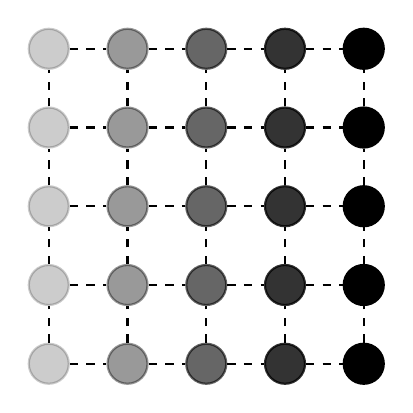
\begin{tikzpicture}[thick]
      \pgfmathsetseed{1}
      \tikzstyle{every node} = [draw, circle, inner sep = 2pt, thick, minimum size=0.2in];


      \onslide<1->{
        \foreach \i in {0,1,2,3,4}{
          \foreach \j in {0,1,2,3,4}{
            \node(\i\j)[fill, opacity=(1+\i)/5] at (\i,\j) {};
          }
        }
      }

      \onslide<3->{
        \path[dashed, thick]
        \foreach \i in {0,1,2,3,4}{
          \foreach \j/\jj in {0/1,1/2,2/3,3/4}{
            (\i\j) edge (\i\jj)
          }
        }
        \foreach \i/\ii in {0/1,1/2,2/3,3/4}{
          \foreach \j in {0,1,2,3,4}{
            (\i\j) edge (\ii\j)
          }
        };
      }
    \end{tikzpicture}};
    }


    \onslide<2->{
      \node at (-4, 0) {Graph:};
      \node[scale=0.8] at (0,0) {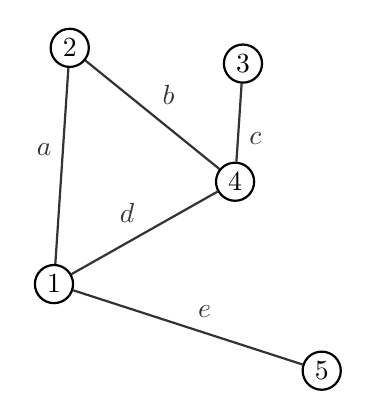
\begin{tikzpicture}[auto]
        \tikzstyle{every node} = [draw, circle, inner sep = 2pt, thick];
        \node(1) at (1,2) {1};
        \node(2) at (1.2,5) {2};
        \node(3) at (3.4,4.8) {3};
        \node(4) at (3.3,3.3) {4};
        \node(5) at (4.4,0.9) {5};
        \tikzstyle{every node} = []
        \path[opacity=0.8,thick]
        (1) edge node[black] {$a$} (2);
        \path[opacity=0.8,thick]
        (2) edge node[black] {$b$} (4);
        \path[opacity=0.8,thick]
        (4) edge node[swap,black] {$c$} (3);
        \path[opacity=0.8,thick]
        (1) edge node[black] {$d$} (4);
        \path[opacity=0.8,thick]
        (1) edge node[black] {$e$} (5);
        \end{tikzpicture}};
      \node at (5,0) {\begin{tikzpicture}[auto]
        \node at (0,1.5) {$\left(\begin{array}{ccccc}
        \0 & a & \0 & d & e\\
        a & \0 & \0 & b & \0\\
        \0 & \0 & \0 & c & \0\\
        d & b & c & \0 & \0\\
        e & \0 & \0 & \0 & \0
        \end{array}\right)$};
        \node at (0,0) {$A$: adjacency matrix};
        \end{tikzpicture}};
    }
  \end{tikzpicture}
\end{center}
\end{figure}
\end{frame}

\begin{frame}[c, label=current]
  \frametitle{Examples of signals}
    \onslide<2>{Most domains can be represented with a graph:\\}
    \begin{center}
    \begin{tikzpicture}
    \node[text width=2cm,align=center] at (-4,4) {Euclidean domains};
    \node[text width=2cm,align=center] at (-4,0) {Non-Euclidean domains};

    \onslide<1>{
    \node at (0, 4) {\includegraphics[width=0.4\linewidth,height=\textheight,keepaspectratio]{cat.jpeg}};
    \node at (5, 4) {\includegraphics[width=0.3\linewidth,height=\textheight,keepaspectratio]{sound.jpeg}};
    }

    \node at (0, 0) {\includegraphics[width=0.4\linewidth,height=\textheight,keepaspectratio]{brain.jpeg}};
    \node at (5, 0) {\includegraphics[width=0.3\linewidth,height=\textheight,keepaspectratio]{social.png}};
    
    \onslide<2>{
    \node at (0, 4) {\includegraphics[width=0.3\linewidth,height=\textheight,keepaspectratio]{grid.pdf}};
    \node at (5, 4) {\includegraphics[width=0.25\linewidth,height=\textheight,keepaspectratio]{line.pdf}};
    }
    \end{tikzpicture}
    \end{center}
\end{frame}

% \begin{frame}[c, label=current]
%   \frametitle{Example of deep learning architecture: VGG-16}
%   \centering\includegraphics[width=0.8\textwidth,height=0.8\textheight,keepaspectratio]{vgg16.png}
% \end{frame}

% \begin{frame}[c, label=current]
%   \frametitle{Another example: Residual Network}
%   \centering\includegraphics[width=\textwidth,height=\textheight,keepaspectratio]{resnet.png}
% \end{frame}

\begin{frame}[c, label=tikz]
  \frametitle{Deep learning performances}
  On Euclidean domains:
    \begin{center}
    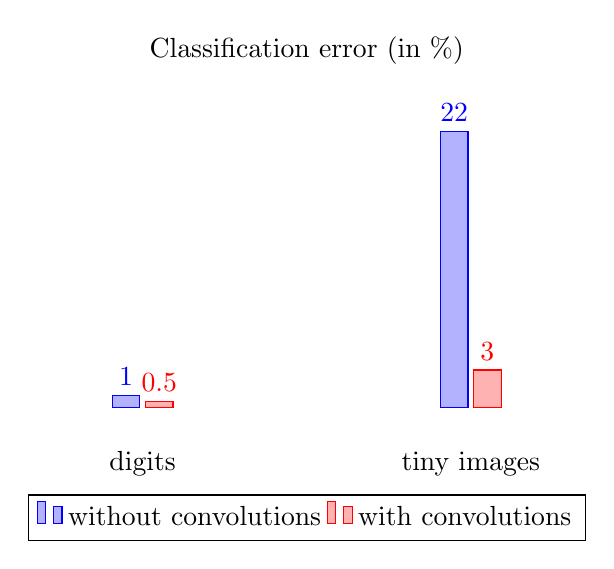
\begin{tikzpicture}
    \begin{axis}[
      title = Classification error (in \%),
      ybar,
      tickwidth = 0,
      x axis line style = { opacity = 0 },
      axis y line       = none,
      enlargelimits=0.15,
      legend style={at={(0.5,-0.15)},
        anchor=north,legend columns=-1},
      ylabel={précision},
      symbolic x coords={digits,tiny images},
      xtick=data,
      nodes near coords,
      nodes near coords align={vertical},
      ]
  \addplot coordinates {(digits,1) (tiny images,22)};
  \addplot coordinates {(digits,0.5) (tiny images,3)};
  \legend{without convolutions, with convolutions}
  \end{axis}
  \end{tikzpicture}
  \end{center}
  % \begin{itemize}
  %   \item MultiLayer Perceptron (MLP): any datasets
  %   \item Convolutional Neural Network (CNN): only Euclidean-structured datasets
  % \end{itemize}
\end{frame}

\begin{frame}[c, label=current]
  \frametitle{A key factor: convolution}
  Defined on Euclidean domains:\\
  \begin{center}
  \includegraphics[width=0.69\textwidth,height=0.69\textheight,keepaspectratio]{conv.png}
  \end{center}
\end{frame}

\begin{frame}[c, label=tikz]
  \frametitle{Connectivity pattern: MLP vs CNN}

  \begin{center}
  \vspace{0.8cm}
    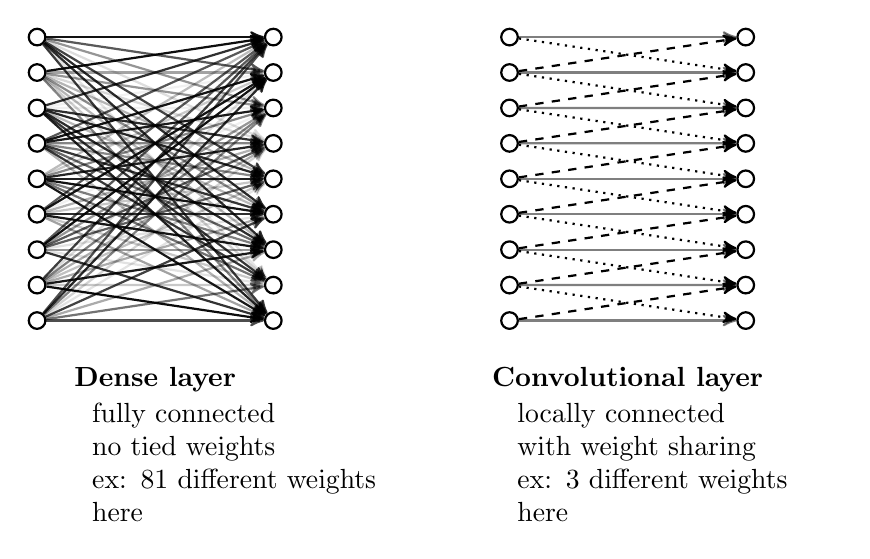
\begin{tikzpicture}[thick,scale=1.5, every node/.style={scale=1.5}]
    \onslide<1->{
      \tikzstyle{every node}=[draw, circle, minimum width=6pt, inner sep = 0pt, thick];
      \foreach \i in {1,...,9}{
        \node(0\i) at (0,.{3*\i}cm) {};}
      \foreach \i in {1,...,9}{
        \node(1\i) at (2,.{3*\i}cm) {};}

      \pgfmathsetseed{2}
      \path[>=stealth',->]
      \foreach \i in {1,...,9}{
        \foreach \j in {1,...,9}{
          (0\i) edge[opacity=(rand+1)/2] (1\j)
        }
      };

      \tikzstyle{every node}=[];
      \node at (1, -0.2) {\textbf{Dense layer}};
      \node[text width=4cm, align=left] at (1.8,-0.9) {fully connected\\ no tied weights\\ ex: 81 different weights here};
    }

    \onslide<2->{
      \tikzstyle{every node}=[draw, circle, minimum width=6pt, inner sep = 0pt, thick];
      \foreach \i in {1,...,9}{
        \node(2\i) at (4,.{3*\i}cm) {};}
      \foreach \i in {1,...,9}{
        \node(3\i) at (6,.{3*\i}cm) {};}
        
      \path[>=stealth',->]
      \foreach \i in {1,...,9}{
      (2\i) edge[opacity=0.5] (3\i)
      };

      \path[>=stealth',->]
      (21) edge[dashed] (32)
      (22) edge[dashed] (33)
      (23) edge[dashed] (34)
      (24) edge[dashed] (35)
      (25) edge[dashed] (36)
      (26) edge[dashed] (37)
      (27) edge[dashed] (38)
      (28) edge[dashed] (39)
      ;

      \path[>=stealth',->]
      (22) edge[dotted] (31)
      (23) edge[dotted] (32)
      (24) edge[dotted] (33)
      (25) edge[dotted] (34)
      (26) edge[dotted] (35)
      (27) edge[dotted] (36)
      (28) edge[dotted] (37)
      (29) edge[dotted] (38)
      ;

      \tikzstyle{every node}=[];
      \node at (5, -0.2) {\textbf{Convolutional layer}};
      \node[text width=4cm, align=left] at (5.4,-0.9) {locally connected\\ with weight sharing\\ ex: 3 different weights here};
    }
    \end{tikzpicture}
  \end{center}
\end{frame}


% \begin{frame}[c, label=current]
%   \frametitle{Non-Euclidean structures}
%   \begin{center}
%   \begin{tikzpicture}
%   \node at (0, 4) {\includegraphics[width=0.4\linewidth,height=\textheight,keepaspectratio]{brain.jpeg}};
%   \node at (5, 4) {\includegraphics[width=0.4\linewidth,height=\textheight,keepaspectratio]{social.png}};
%   \node at (0, 0) {\includegraphics[width=0.4\linewidth,height=\textheight,keepaspectratio]{sen.jpg}};
%   \node at (5, 0) {\includegraphics[width=0.4\linewidth,height=\textheight,keepaspectratio]{plane.png}};
%   \end{tikzpicture}
%   \end{center}
% \end{frame}


\begin{frame}[c, label=tikz]
  \frametitle{Problem: How to extend convolutions?}
  
\begin{center}

    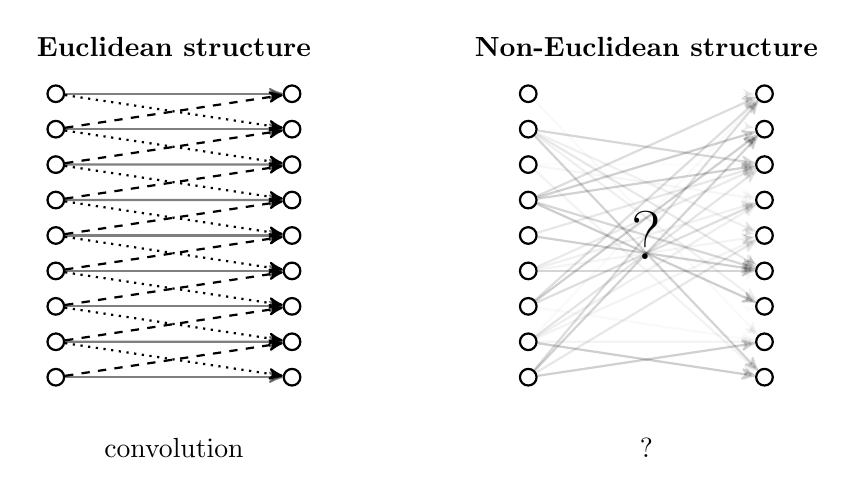
\begin{tikzpicture}[thick,scale=1.5, every node/.style={scale=1.5}]
      \tikzstyle{every node}=[];
      \node at (1, 3.1) {\textbf{Euclidean structure}};
      \node at (5, 3.1) {\textbf{Non-Euclidean structure}};

      \tikzstyle{every node}=[draw, circle, minimum width=6pt, inner sep = 0pt, thick];

      \foreach \i in {1,...,9}{
        \node(2\i) at (0,.{3*\i}cm) {};}
      \foreach \i in {1,...,9}{
        \node(3\i) at (2,.{3*\i}cm) {};}

      \foreach \i in {1,...,9}{
        \node(4\i) at (4,.{3*\i}cm) {};}
      \foreach \i in {1,...,9}{
        \node(5\i) at (6,.{3*\i}cm) {};}

      %\pause
        
      \path[>=stealth',->]
      \foreach \i in {1,...,9}{
      (2\i) edge[opacity=0.5] (3\i)
      };

      \path[>=stealth',->]
      (21) edge[dashed] (32)
      (22) edge[dashed] (33)
      (23) edge[dashed] (34)
      (24) edge[dashed] (35)
      (25) edge[dashed] (36)
      (26) edge[dashed] (37)
      (27) edge[dashed] (38)
      (28) edge[dashed] (39)
      ;

      \path[>=stealth',->]
      (22) edge[dotted] (31)
      (23) edge[dotted] (32)
      (24) edge[dotted] (33)
      (25) edge[dotted] (34)
      (26) edge[dotted] (35)
      (27) edge[dotted] (36)
      (28) edge[dotted] (37)
      (29) edge[dotted] (38)
      ;

      \tikzstyle{every node}=[];
      \node at (1, -0.3) {convolution};

      \pause

      \pgfmathsetseed{1}
        \path[>=stealth',->]
        \foreach \i in {1,...,9}{
          \foreach \j in {1,...,9}{
            (4\i) edge[opacity=0.2*rand] (5\j)
          }
        };

      \tikzstyle{every node}=[];
      \node at (5, 1.5cm) {\Huge?};
      \node at (5, -0.3) {?};
    \end{tikzpicture}
  \end{center}
\end{frame}

\begin{frame}[c, label=current]
  \frametitle{Supervised vs semi-supervised application}
  Let $X$ be a dataset. We classify its rows. Two different kind of graph structures:
  \begin{center}
  \begin{tikzpicture}
  \node[text width=2cm,align=center] at (-4, 4) {Supervised classification of graph-structured data};
  \node at (0, 4) {\includegraphics[width=0.4\linewidth,height=\textheight,keepaspectratio]{brain.jpeg}};
  \node at (5, 3.7) {$\matbox{7}{4}{b}{n}{X}$};
  \path[color=red, <->, thick] (4.2,5.4) edge (5.8,5.4);
  \node at (5, 5.6) {$\textcolor{orange}{n}$};
  \node[text width=2cm,align=center] at (-4, 0) {Semi-supervised classification of nodes};
  \node at (0, 0) {\includegraphics[width=0.32\linewidth,height=\textheight,keepaspectratio]{social.png}};
  \node at (5, 0) {$\matbox{4}{7}{n}{p}{X}$};
  \path[color=red, <->, thick] (3.4,-0.6) edge (3.4,0.88);
  \node at (3.2, 0.15) {$\textcolor{orange}{n}$};
  \end{tikzpicture}
  \end{center}
\end{frame}


\section{Literature overview}


\begin{frame}[c, label=current]
  \frametitle{Spectral approaches}
  Convolutions are defined in the graph spectral domain.
  \begin{Large}
  $$
  L = D - A = U \Lambda U^T \quad \quad \quad \textsc{gft}(X) = UX
  $$
  \end{Large}
  \vspace{-0.4in}
  \begin{figure}
  \begin{center}
  \includegraphics[width=0.8\linewidth,height=\textheight,keepaspectratio]{mines2.png}\\
  \end{center}
  \caption{Example of signals of the Laplacian eigenbasis}
  \end{figure}
  Using the GFT, convolution amount to a pointwise multiplication in the spectral domain.
  \begin{Large}
  $$
  X \otimes \Theta = U^T(UX . U\Theta)
  $$
  \end{Large}
\end{frame}


\begin{frame}[c, label=current]
  \frametitle{Spectral approaches}
  \begin{Large}
  $$
  X \otimes \Theta = U^T(UX . U\Theta)
  $$
  \end{Large}
  Pros\\
  \begin{itemize}
  \item Elegant and fast under some approximations
  \item Can be used off the shelf: no need to specify any weight sharing
  \end{itemize}
  Cons\\
  \begin{itemize}
  \item Introduce isotropic symmetries
  \item Do not match Euclidean convolutions on grid graphs
  \end{itemize}
  %\vspace{-0.3in}
  \begin{figure}
  \begin{center}
  \includegraphics[width=0.2\textwidth,height=\textheight,keepaspectratio]{before_trans.png}
  \hspace{0.5in}
  \includegraphics[width=0.2\textwidth,height=\textheight,keepaspectratio]{after_trans.png}
  \end{center}
  \caption{Example of translation defined as convolution with a dirac (courtesy of Pasdeloup, B.)}
  \end{figure}
\end{frame}

\begin{frame}[c, label=current]
  \frametitle{Vertex-domain approaches}
  Convolutions are defined as a sum over a neighborhood, usually a sum of dot products (cf references in thesis manuscript).
  \begin{Large}
  $$
  (X \otimes \Theta)(v_i) = \sum_{j \in \mathcal{N}_{v_i}}{\theta_{ij}X(v_j)}
  $$
  \end{Large}

  \begin{figure}
  \begin{center}
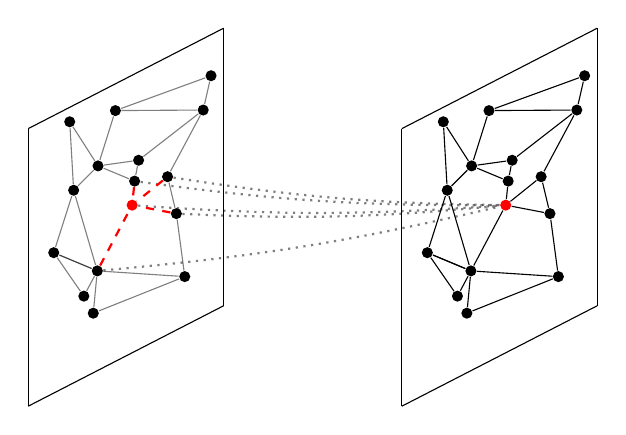
\begin{tikzpicture}[scale=0.75]
  
\newcommand{\nnn}{4.7}
  \begin{scope}[rotate around y = 70]
\pgfmathsetseed{333}
\tikzstyle{every node}= [circle,
fill=black,
 minimum size= 4pt,inner sep=0pt];
    \foreach \x in {1,2,4}{
      \foreach \y in {1,2,3,4}{
        \node(\x\y) at (\x+0.5*rand,\y+0.5*rand) {};
      }
    }
    \foreach \y in {1,2,4}{
        \node(3\y) at (3+0.5*rand,3+0.5*rand) {};
    }
    \node(33)[circle,fill=red] at (2.5,2.5) {};

    \path[thin]
      (0,0) edge (0,\nnn)
      (0,\nnn) edge (\nnn,\nnn)
      (0,0) edge (\nnn,0)
      (\nnn,0) edge (\nnn,\nnn);

    %\node[draw=none,fill=none] at (2.8,-1) {$V_\pi$};
    \end{scope}
  \begin{scope}[xshift=180pt,rotate around y = 70]
\pgfmathsetseed{333}
\tikzstyle{every node}= [circle,fill=black, minimum size= 4pt,inner sep=0pt];
    \foreach \x in {1,2,4}{
      \foreach \y in {1,2,3,4}{
        \node(\x\y') at (\x+0.5*rand,\y+0.5*rand) {};
      }
    }
    \foreach \y in {1,2,4}{
        \node(3\y') at (3+0.5*rand,3+0.5*rand) {};
    }
    \node(33')[circle,fill=red] at (2.5,2.5) {};

    \path[thin]
      (0,0) edge (0,\nnn)
      (0,\nnn) edge (\nnn,\nnn)
      (0,0) edge (\nnn,0)
      (\nnn,0) edge (\nnn,\nnn);

    %\node[draw=none,fill=none] at (2.8,-1) {$U$};
  \end{scope}

\draw[dotted,thick,-,opacity=0.5] (33) edge[bend right=4] (33');
\draw[dotted,thick,-,opacity=0.5] (22) edge[bend right=4] (33');
\draw[dotted,thick,-,opacity=0.5] (32) edge[bend right=4] (33');
\draw[dotted,thick,-,opacity=0.5] (31) edge[bend right=4] (33');
\draw[dotted,thick,-,opacity=0.5] (42) edge[bend right=4] (33');

\path[thick, dashed, red]
  (22) edge (33)
  (32) edge (33)
  (31) edge (33)
  (42) edge (33);

\path[opacity=0.5]
  (22) edge (13)
  (22) edge (12)
  (22) edge (11)
  (22) edge (21)
  (22) edge (41)
  (21) edge (41)
  (42) edge (31)
  (43) edge (31)
  (43) edge (24)
  (44) edge (43)
  (32) edge (23)
  (32) edge (34)
  (22) edge (12)
  (23) edge (14)
  (11) edge (12)
  (14) edge (13)
  (24) edge (23)
  (34) edge (43)
  (23) edge (34)
  (23) edge (13)
  (12) edge (13)
  (42) edge (41)
  (24) edge (44);

\path[]
  (22') edge (33')
  (32') edge (33')
  (31') edge (33')
  (42') edge (33')
  (22') edge (13')
  (22') edge (12')
  (22') edge (11')
  (22') edge (21')
  (22') edge (41')
  (21') edge (41')
  (42') edge (31')
  (43') edge (31')
  (43') edge (24')
  (44') edge (43')
  (32') edge (23')
  (32') edge (34')
  (22') edge (12')
  (23') edge (14')
  (11') edge (12')
  (14') edge (13')
  (24') edge (23')
  (34') edge (43')
  (23') edge (34')
  (23') edge (13')
  (12') edge (13')
  (42') edge (41')
  (24') edge (44');

\end{tikzpicture}
  \end{center}
  %\caption{An LRF of a vertex (in red) of an EC layer}
  %\label{fig:lrf}
\end{figure}

\end{frame}

\begin{frame}[c, label=current]
  \frametitle{Vertex-domain approaches}
  \begin{Large}
  $$
  (X \otimes \Theta)(v_i) = \sum_{j \in \mathcal{N}_{v_i}}{\theta_{ij}X(v_j)}
  $$
  \end{Large}
  Pros
  \begin{itemize}
  \item Match Euclidean convolutions on grid graphs
  \item Locally connected
  \end{itemize}
  Cons
  \begin{itemize}
  \item Weight sharing is not always explicit
  \end{itemize}
  \centering\includegraphics[width=0.4\linewidth,height=\textheight,keepaspectratio]{gridDeformed}
\end{frame}

\begin{frame}[c, label=current]
  \frametitle{A few important references}
  \begin{itemize}
    \item Bruna et al., 2013: spectral filters with $\mathcal{O}(1)$ weights, $K$ smoother matrix used to interpolate more weights.
    $$
    g_\theta(X) = U^T(UX . K\theta)
    $$
    \item Defferard et al., 2016: filters based on Chebychev polynomials $(T_i)_i$.
    $$
    g_\theta(L) = \sum_{i=0}^k \theta_i \h{2} T_i(\widetilde{L})
    $$
    \item Kipf et al., 2016: application to semi-supervised settings.
    $$
    Y = \widetilde{A} X \Theta \label{eq:gcn}
    $$
    \item Velickovic et al., 2017: introduction of attention coefficients $(A_k)_k$.
    $$
    Y = \displaystyle\bigparallel_{k=1}^K A_k X \Theta_k
    $$
    \item Du et al., 2017: convolution from  the GSP field (Sandryhaila et al., 2013).
    $$
    Y = \sum_{k=1}^K \widetilde{A}^k X \Theta_k
    $$
  \end{itemize}
\end{frame}


\section{Convolution of graph signals}


\begin{frame}[c, label=current]
  \frametitle{Recall: Euclidean convolution}
  \begin{definition}\textbf{Convolution on $\cs(\bbz^2)$}\\
  The (discrete) convolution $s_1 \ast s_2$ is a binary operation in $\cs(\bbz^2)$ defined as:
  \begin{align*}
  \forall (a,b) \in \bbz^2, (s_1 \ast s_2) [a,b] & = \displaystyle \sum_i \sum_j s_1[i,j] \h{2} s_2[a-i, b-j]
  \end{align*}
  A convolution operator $f$ is a function parameterized by a signal $w \in \cs(\bbz^2)$ \st:
    \begin{itemize}
      \item $f = . \ast w$ (right operator)
      \item $f = w \ast .$ (left operator)
    \end{itemize}
  \label{def:conv}
  \end{definition}

Some notable properties:
  \begin{itemize}
    \item Linearity
    \item Locality and weight sharing
    \item Commutativity (optional)
    \item Equivariance to translations (\ie commutes with them)
  \end{itemize}
\end{frame}

\begin{frame}[c, label=current]
  \frametitle{Characterization by translational equivariance}

  % \begin{itemize}
  % \item We propose to extend convolutions to graph signals while preserving the following characterization:
  % \end{itemize}

  \begin{theorem}\textbf{Characterization of convolution operators on $\cs(\bbz^2)$}\\
  A linear transformation $f$ is equivariant to translations $\Leftrightarrow$ it is a convolution operator.
  \label{prop:equi}
  \end{theorem}

  \begin{figure}
  \begin{tikzpicture}
  \node(a) at (0, 3) {\includegraphics[width=0.22\linewidth,height=\textheight,keepaspectratio]{cat.jpeg}};
  \node(b) at (6, 3) {\includegraphics[width=0.22\linewidth,height=\textheight,keepaspectratio]{cat_translated.jpeg}};
  \node(c) at (0, 0) {\includegraphics[width=0.22\linewidth,height=\textheight,keepaspectratio]{cat_filtered.jpeg}};
  \node(d) at (6, 0) {\includegraphics[width=0.22\linewidth,height=\textheight,keepaspectratio]{cat_translated_filtered.jpeg}};
  \path[->, thick] (a) edge node[above] {\textit{translation}} (b);
  \path[->, thick] (a) edge node[left] {\scalebox{1.32}{$f$}} (c);
  \path[->, thick] (b) edge node[right] {\scalebox{1.32}{$f$}} (d);
  \path[->, thick] (c) edge node[above] {\textit{translation}} (d);
  \end{tikzpicture}
  \end{figure}

\end{frame}

\begin{frame}[c, label=tikz]
  \frametitle{Convolution of signals with graph domains}
  \begin{columns}
    \column{.5\textwidth}
    \begin{center}
      \scalebox{0.9}
      {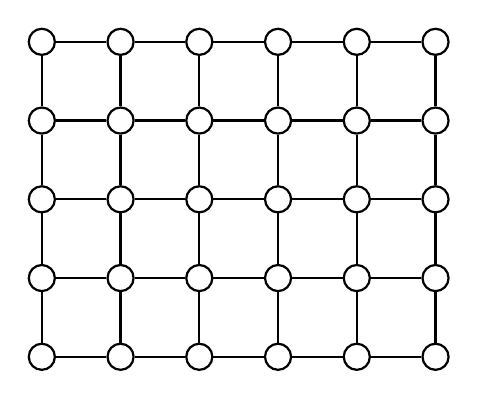
\begin{tikzpicture}[thick]
              \tikzstyle{every node} = [draw, circle];
              \foreach \i in {0,1,2,3,4,5}{
                \foreach \j in {0,1,2,3,4}{
                  \node(\i\j) at (\i,\j) {};
                }
              }
              \path[]
              \foreach \i in {0,1,2,3,4,5}{
                \foreach \j/\jj in {0/1,1/2,2/3,3/4}{
                  (\i\j) edge (\i\jj)
                }
              }
              \foreach \i/\ii in {0/1,1/2,2/3,3/4,4/5}{
                \foreach \j in {0,1,2,3,4}{
                  (\i\j) edge (\ii\j)
                }
              };
            \end{tikzpicture}}
      \h{0}\\Can use the Euclidean convolution
    \end{center}
    \column{.5\textwidth}
    \begin{center}
    \scalebox{0.9}
      {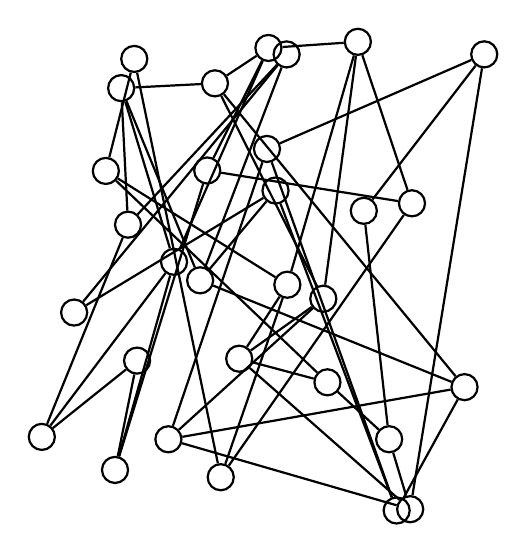
\begin{tikzpicture}[thick]
              \tikzstyle{every node} = [draw, circle];
              \foreach \i in {0,1,2,3,4,5}{
                \foreach \j in {0,1,2,3,4}{
                  \node(\i\j) at (3+3*rand,3+3*rand) {};
                }
              }
              \path[]
              \foreach \i in {0,1,2,3,4,5}{
                \foreach \j/\jj in {0/1,1/2,2/3,3/4}{
                  (\i\j) edge (\i\jj)
                }
              }
              \foreach \i/\ii in {0/1,1/2,2/3,3/4,4/5}{
                \foreach \j in {0,1,2,3,4}{
                  (\i\j) edge (\ii\j)
                }
              };
            \end{tikzpicture}}
      \h{0}\\How to extend the convolution here ?
    \end{center}
  \end{columns}
\end{frame}

\begin{frame}[c, label=current]
  \frametitle{A few notions of representation theory}
  A group is a set (defined by some properties) which can act on other sets.\\
  \h{0}\\
  Let $\Gamma$ be a group, $g \in \Gamma$, and $V$ be a set. Example of group actions:
  \begin{itemize}
    \item $L_g: \Gamma \to \Gamma$ (auto-action)
    \item $g(.): V \to V$ (action on $V$)
  \end{itemize}

  \begin{figure}\scalebox{1.7}{
  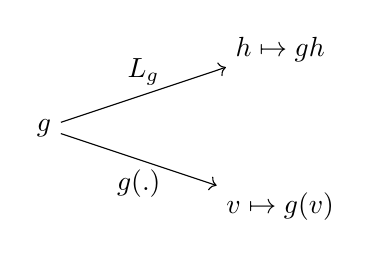
\begin{tikzpicture}
  \node(a) at (0,0) {$g$};
  \node(b) at (3,1) {$h \mapsto gh$};
  \node(c) at (3,-1) {$v \mapsto g(v)$};
  \path[->] (a) edge node[above] {$L_g$} (b);
  \path[->] (a) edge node[below] {$g(.)$} (c);
  \end{tikzpicture}
  }
  \end{figure}
%   \begin{definition}\textbf{Group}\\
%   A group $\Gamma$ is a set equipped with a closed, associative and invertible composition law that admits a unique left-right identity element. When the law is commutative, the group is said to be \emph{abelian}.
%   \end{definition}
  
%   \begin{lemma}\textbf{Symmetric group}\\
%     Let a set $V$. The set of its bijective transformations $\Phi^*(V)$ forms a group called its symmetric group.
%   \end{lemma}

%   A group is an object that can act on a set:

%   \begin{definition}\textbf{Group action}\\
%     An \emph{action} of a group $\Gamma$ on a set $V$ is a homomorphism $L: \Gamma \to \Phi^*(V)$.
%   \end{definition}
\end{frame}

\begin{frame}[c, label=current]
  \frametitle{Group convolution}
    \begin{definition}\textbf{Group convolution}\\
    Let a group $\Gamma$, the group convolution between two signals $s_1$ and $s_2 \in \cs(\Gamma)$ is defined as:
    \begin{align*}
    \forall h \in \Gamma, (s_1 \ast_{\I} s_2)[h] & = \displaystyle \sum_{g \in \Gamma} s_1[g] \h{2} s_2[g^{-1}h]%\\
    %& = \displaystyle \sum_{ab = h} s_1[a] \h{2} s_2[b]
    \end{align*}
    provided at least one of the signals has finite support if $\Gamma$ is not finite.
    \label{def:conv1}
    \end{definition}

    \begin{theorem}\textbf{Characterization of group convolution operators}\\
    Let a group $\Gamma$, let $f \in \cl(\cs(\Gamma))$,
    \begin{enumerate}%[nolistsep,noitemsep,label=(\roman*)]
      \item $f$ is a group convolution right operator $\Leftrightarrow$ $f$ is equivariant to left multiplications, %\label{enum:p}
      \item $f$ is a group convolution left operator $\Leftrightarrow$ $f$ is equivariant to right multiplications, %\label{enum:pp}
      \item $f$ is a group convolution commutative operator $\Leftrightarrow$ $f$ is equivariant to multiplications. %\label{enum:ppp}%$\Leftrightarrow$ $\Gamma$ is abelian \label{enum:ppp}
    \end{enumerate}
    %\label{th:cgco}
    \end{theorem}
\end{frame}

% \begin{frame}[c, label=current]
%   \frametitle{Graphs and linear extension of transformations}
  
%   \begin{definition}\textbf{Graph}\\
%   A \emph{graph} $G$ is a couple of countable vertex and edge sets $\langle V,E \rangle$ \st $E \subset V^2$.
%   \end{definition}

%   %\pause

%   % \begin{definition}\textbf{Transformation and group action}\\
%   % A \emph{transformation} $f: V \rightarrow V$ is a function with same domain and codomain.\\
%   % The set of bijective transformations, called the \emph{symmetric group}, is denoted $\Phi^*(V)$.\\
%   % An \emph{action} of a group $\Gamma$ on a set $V$ is a homomorphism $L: \Gamma \to \Phi^*(V)$.
%   % \end{definition}

%   %A transformation is an action of an element of a group.
%   %\pause

%   A bijective transformation of a vertex set $V$ can be extended to graph signals of $\cs(V)$.

%   \begin{lemma}\textbf{Extension of bijective transoformations to signals}\\
%   A bijective transformation $f \in \Phi^*(V)$ can be extended linearly to the signal space $\cs(V)$, and we have:
%   \begin{gather*}
%   \forall s \in \cs(V), \forall v \in V, f(s)[v] = s[f^{-1}(v)]
%   \end{gather*}
%   \label{lem:extlin}
%   \end{lemma}
% \end{frame}

\begin{frame}[c, label=current]
  \frametitle{Goal: convolution on the vertex set}
  %\only<5->{

    Let a graph $G = \langle V,E \rangle$ \st $E \subset V^2$.\\
    Starting point: bijective map $\varphi$ between a group $\Gamma$ and $G$ (or a subgraph).
    \begin{figure}
    \scalebox{2.}
    {\begin{tikzcd}[ampersand replacement=\&]
            \Gamma \arrow{r}{\varphi}  \arrow{d}[swap]{\text{lin. ext.}}  \& V \arrow{d}{\text{lin. ext.}}\\  
            \cs(\Gamma) \arrow{r}[swap]{\widetilde\varphi}  \& \cs(V) 
        \end{tikzcd}}
    %\caption{Commutative diagram}
    \end{figure}
   
  %}
  % \begin{itemize}
  %   \item<1-> a graph $\gve$ (or subgraph)
  %   \item<2-> a subgroup $\Gamma$ of the symmetric group of $V$
  %   \item<3-> such that there exists a one-to-one correspondence $\varphi: \Gamma \to V$
  %   \item<4-> $\varphi$ defines by linear extension from dirac bases $\widetilde\varphi: \cs(\Gamma) \to \cs(V)$
  %   %\item<5-> denote $g_v = \varphi^{-1}(v)$  
  % \end{itemize}
\end{frame}

\begin{frame}[c, label=current]
  \frametitle{Convolution on the vertex set from group convolutions}
  (Goal: convolution on the vertex set)\\
  $\varphi$: bijective map
    \begin{figure}
    \scalebox{1.9}
    {\begin{tikzcd}[ampersand replacement=\&]%
    \cs(\Gamma) \arrow{d}[swap]{\widetilde f} \& \cs(V) \arrow{d}{f =\varphi \circ \widetilde{f} \circ \varphi^{-1}} \arrow{l}[swap]{\varphi^{-1}}\\
    \cs(\Gamma) \arrow{r}[swap]{\varphi} \& \cs(V)
\end{tikzcd}}
    %\caption{Commutative diagram}
    \end{figure}
    %$f$ is characterized by equivariance to $\varphi \circ L_\Gamma \circ \varphi^{-1}$, where $L_\Gamma$ is left multiplication auto-action.\\
    %We want characteirzation by equivariance to $\Gamma$.
    Equivariance theorem to operators of the form $\varphi \circ L_g \circ \varphi^{-1}$ holds.\\
    But not necessarily to actions of $\Gamma$ on $V$ (\ie of the form $g(.)$).
\end{frame}

\begin{frame}[c, label=current]
  \frametitle{Needed condition: equivariant map}
  (Goal: equivariance theorem holds)\\
  Condition: $\varphi$ is a bijective equivariant map\\
  Denote $g_v = \varphi^{-1}(v)$.
    \begin{figure}
    \scalebox{2.}
    {
\begin{tikzcd}[ampersand replacement=\&]
    g_u \arrow{r}{L_{g_v}}  \arrow{d}[swap]{\varphi}  \& g_vg_u \arrow{d}{\varphi}\\  
    u \arrow[dashrightarrow, red]{r}{}[below]{g_v(.)}  \& \varphi(g_vg_u)
\end{tikzcd}}
    %\caption{Commutative diagram}
    \end{figure}
    We need $\textcolor{red}{g_v(.)} = \varphi \circ L_{g_v} \circ \varphi^{-1}$\\
    \ie $\forall u \in V, g_v(u) = \varphi(g_v g_u)$.
\end{frame}

\begin{frame}[c, label=current]
  \frametitle{$\varphi$-convolution}
  $\varphi$: bijective equivariant map \ie $g_v(u) = \varphi(g_v g_u)$.
  \begin{definition}\textbf{$\varphi$-convolution}\\
  $\forall s_1, s_2 \in \cs(V)$:
  \begin{align}
  s_1 \ast_{\varphi} s_2 & = \displaystyle \sum_{v \in V} s_1[v] \h{2} g_v(s_2)\label{eq:vdom}\\
  & = \displaystyle \sum_{g \in \Gamma} s_1[\varphi(g)] \h{2} g(s_2) \label{eq:premix}
  \end{align}
  %where $g_v(u) = \varphi(g_v g_u)$.
  %\label{def:conv3}
  \end{definition}
%\end{frame}

%\begin{frame}[c, label=current]
%  \frametitle{Characterization}
\begin{theorem}\textbf{Characterization of $\varphi$-convolution right operators}\\
%Let a group $\Gamma$ acting on $V~\st \Gamma \overset{\varphi}{\equiv} V$, let $f \in \cl(\cs(\Gamma))$, then:\\
\centerline{$f$ is a $\varphi$-convolution right operator $\Leftrightarrow$ $f$ is equivariant to $\Gamma$}
\label{prop:equiG}
\end{theorem}

% \begin{corollary}\textbf{Characterization of $\varphi$-convolution operators}\\
% %Let a group $\Gamma$ acting on $V~\st \Gamma \overset{\varphi}{\equiv} V$\\
% \begin{tabular}{rl}
%   $f$ is equivariant to $\Gamma$ $\Leftrightarrow$ &
%   $f$ is a $\varphi$-convolution operator \st its laterality is \\
%   & opposed to the laterality of the $\varphi$-equivalence
% \end{tabular}
% \label{cor:equiG}
% \end{corollary}

\end{frame}


\begin{frame}[c, label=current]
  \frametitle{Mixed domain formulation}
  Let $\Gamma$ be an abelian group. No need to exhibit $\varphi$ in this case:
  \begin{definition}\textbf{Mixed domain convolution}\\
  $\forall r \in \cs(\Gamma)$ and $\forall s \in \cs(V)$:
  \begin{gather*}
  r \ast_{\M} s = \displaystyle \sum_{g \in \Gamma} r[g] \h{2} g(s) \in \cs(V)
  \end{gather*}
  %Worth noting that $r \ast_{\M} s \in \cs(V)$.
  \label{def:convm}
  \end{definition}
%\pause
  Equivariance theorem holds:
  \begin{corollary}$f$ is a $\M$-convolution left operator $\Leftrightarrow$ $f$ is equivariant to $\Gamma$
  \end{corollary}
  (Converse sense still requires bijectivity between $\Gamma$ and $V$).
%\pause
\end{frame}

% \begin{frame}[c, label=current]
%   \frametitle{Inclusion and role of the edge set}
%   \begin{definition}\textbf{Edge-constrained transformation}\\
%   An \emph{edge-constrained} (EC) transformation on a graph $\gve$ is a transformation $f: V \mapsto V$ such that
%   \begin{gather*}
%   \forall u,v \in V, f(u) = v \Rightarrow u \overset{E}{\sim} v
%   \end{gather*}
%   \end{definition}
% %\pause
%   \begin{definition}\textbf{Edge-constrained convolution}\\
%   A $\varphi$- or $\M$-convolution is said to be EC if $\Gamma$ can be generated from a subset of EC transformations.
%   \end{definition}
% %\pause
%   \begin{definition}\textbf{Locality-preserving convolution}\\
%   A $\varphi$- or $\M$-convolution is said to be LP if actions of $\Gamma$ on $V$ are graph automorphisms.
%   \end{definition}
% \end{frame}

\begin{frame}[c, label=current]
  \frametitle{Inclusion and role of the edge set}
  \begin{itemize}
  \item \textbf{Edge constrained (EC)}\\\h{0}\\
  \begin{figure}
    \begin{center}
      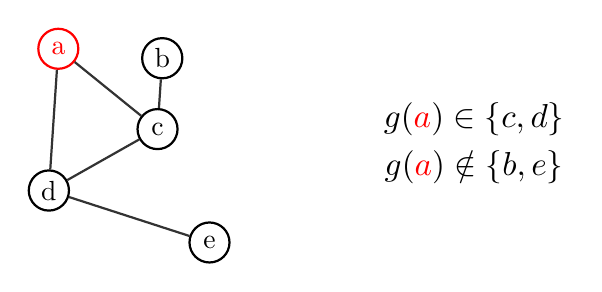
\begin{tikzpicture}[scale=0.6]
          \tikzstyle{every node} = [draw, circle, inner sep = 2pt, thick, minimum size=0.2in];
          \node(1) at (1,2) {d};
          \node[color=red](2) at (1.2,5) {\textcolor{red}{a}};
          \node(3) at (3.4,4.8) {b};
          \node(4) at (3.3,3.3) {c};
          \node(5) at (4.4,0.9) {e};
          \tikzstyle{every node} = []
          \path[opacity=0.8,thick]
          (1) edge (2);
          \path[opacity=0.8,thick]
          (2) edge (4);
          \path[opacity=0.8,thick]
          (4) edge (3);
          \path[opacity=0.8,thick]
          (1) edge (4);
          \path[opacity=0.8,thick]
          (1) edge (5);
          \tikzstyle{every node} = []
          \node at (10,3.5) {\scalebox{1.2}{$g(\textcolor{red}{a}) \in \{c,d\}$}};
          \node at (10,2.5) {\scalebox{1.2}{$g(\textcolor{red}{a}) \notin \{b,e\}$}};
          \end{tikzpicture}
    \end{center}
  \end{figure}

  \item \textbf{Locality Preserving (LP)}\\
  \begin{figure}
    \begin{center}
      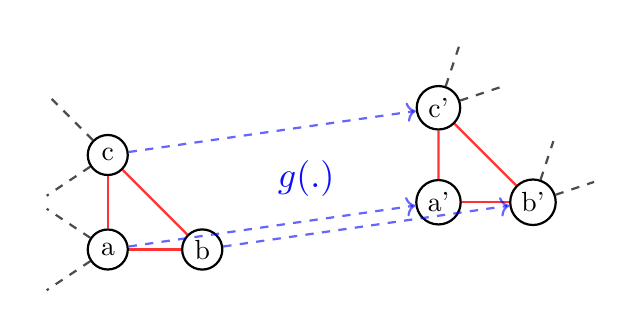
\begin{tikzpicture}[scale=0.6]
          \tikzstyle{every node} = [draw, circle, inner sep = 2pt, thick, minimum size=0.2in];
          \node(1) at (0,0) {a};
          \node(2) at (2,0) {b};
          \node(3) at (0,2) {c};

          \node(4) at (7,1) {a'};
          \node(5) at (9,1) {b'};
          \node(6) at (7,3) {c'};

          \path[opacity=0.8,thick,red] (1) edge (2);
          \path[opacity=0.8,thick,red] (1) edge (3);
          \path[opacity=0.8,thick,red] (2) edge (3);

          \path[opacity=0.8,thick,red] (4) edge (5);
          \path[opacity=0.8,thick,red] (4) edge (6);
          \path[opacity=0.8,thick,red] (5) edge (6);

          \tikzstyle{every node} = []
          \node(7) at (-1.5,3.5) {\h{0}};
          \path[opacity=0.7,thick, dashed] (3) edge (7); 
          \node(8) at (-1.5, 1) {\h{0}};
          \path[opacity=0.7,thick, dashed] (3) edge (8);

          \node(9) at (-1.5,1) {\h{0}};
          \path[opacity=0.7,thick, dashed] (1) edge (9); 
          \node(10) at (-1.5, -1) {\h{0}};
          \path[opacity=0.7,thick, dashed] (1) edge (10);

          \node(13) at (8.5,3.5) {\h{0}};
          \path[opacity=0.7,thick, dashed] (6) edge (13); 
          \node(14) at (7.5,4.5) {\h{0}};
          \path[opacity=0.7,thick, dashed] (6) edge (14);

          \node(17) at (10.5,1.5) {\h{0}};
          \path[opacity=0.7,thick, dashed] (5) edge (17); 
          \node(18) at (9.5,2.5) {\h{0}};
          \path[opacity=0.7,thick, dashed] (5) edge (18);

          \path[opacity=0.6,thick,dashed,->,blue] (1) edge (4);
          \path[opacity=0.6,thick,dashed,->,blue] (2) edge (5);
          \path[opacity=0.6,thick,dashed,->,blue] (3) edge (6);
          \node[opacity=0.95] at (4.2,1.5) {\scalebox{1.3}{$\textcolor{blue}{g(.)}$}};
          \end{tikzpicture}
    \end{center}
  \end{figure}

\end{itemize}
\end{frame}

\begin{frame}[c, label=current]
  \frametitle{Cayley graphs}
  (Goal: description of EC and LP convolutions)\\\h{0}\\
  \begin{definition}\textbf{Cayley graph and subgraph}\\
  Let a group $\Gamma$ and one of its generating set $\cu$. The \emph{Cayley graph} generated by $\cu$, is the digraph $\vgve$ such that $V = \Gamma$ and $E$ is such that, either:
  \begin{itemize}
  \item $\forall a,b \in \Gamma, a \rightarrow b \Leftrightarrow \exists g \in \cu, ga = b \quad$ (\emph{left Cayley graph})
  \item $\forall a,b \in \Gamma, a \rightarrow b \Leftrightarrow \exists g \in \cu, ag = b \quad$ (\emph{right Cayley graph})
  \item both points above (\emph{abelian Cayley graph})
  \end{itemize}
  %\only<4->{
  A \emph{Cayley subgraph} is a subgraph that is isomorph to a Cayley graph.
  %}
  \end{definition}

  \begin{figure}
  \begin{center}
  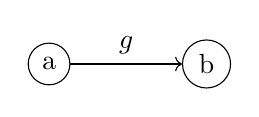
\begin{tikzpicture}
  \tikzstyle{every node} = [draw, circle, inner sep = 3pt]
      \node(a) at (0,0) {a};
      \node(b) at (2,0) {b};
  \tikzstyle{every node} = []
      \path[->] (a) edge node[above] {$g$} (b);
  \end{tikzpicture}
  \end{center}
  \caption{An edge of a Cayley graph}
  \end{figure}

  % \begin{theorem}\textbf{Characterization by Cayley subgraphs}\\
  % Let a graph $\gve$, then:
  % \begin{enumerate}
  % \item its left Cayley subgraphs characterize its EC equivariant $\varphi$-convolutions
  % \item its right Cayley subgraphs characterize its LP equivariant $\varphi$-convolutions
  % \item its abelian Cayley subgraphs characterize its EC and LP equivariant $M$-convolutions
  % \end{enumerate}
  % \label{th:cayleychar}
  % \end{theorem}
\end{frame}

\begin{frame}[c, label=current]
  \frametitle{Characterization of EC and LP convolutions}
  \begin{theorem}\textbf{Characterization by Cayley subgraphs}\\
  Let a graph $\gve$, then:
  \begin{enumerate}
  \item its left Cayley subgraphs characterize its EC $\varphi$-convolutions,
  \item its right Cayley subgraphs characterize its LP $\varphi$-convolutions,
  \item its abelian Cayley subgraphs characterize its EC and LP $\M$-convolutions.
  \end{enumerate}
  \label{th:cayleychar}
  \end{theorem}

  \begin{corollary}\textbf{Properties of convolutions that are both EC and LP}\\
  \begin{enumerate}
  \item If a $\varphi$-convolution of group $\Gamma$ is EC and LP then $\Gamma$ is abelian;
  \item an $\M$-convolution is EC if, and only if, it is also LP.
  \end{enumerate}
  \end{corollary}
\end{frame}

\begin{frame}[c, label=current]
  \frametitle{Other results in the manuscript}
\begin{itemize}
    \item Description with smaller kernels
    \item The weight sharing is preserved
    \item More detailed results depending on laterality of operator and equivariance
    \item Analysis of limitations due to algebraic structure of the Cayley subgraphs
    \item Above theorems hold for groupoids of partial transformation under mild conditions
    \item They also hold for groupoids based on paths under restrictive conditions
  \end{itemize}
\end{frame}

\section{Deep learning on graph domains}

\begin{frame}[c, label=current]
  \frametitle{Propagational representation of a layer}
  \begin{figure}
  \centering\includegraphics[width=0.51\linewidth,height=\textheight,keepaspectratio]{graphFig.pdf}
  %\caption{Local receptive field (LRF), in red, of a neuron on the left layer}
  \end{figure}

  % \begin{definition}\textbf{Edge-constrained layer}\\
  % A layer $\cl: \gve \rightarrow U$, is said to be \emph{edge-constrained} (EC) if:
  % \begin{enumerate}
  % \item There is a one-to-one correspondence $\pi: V_\pi \rightarrow U$, where $V_\pi \subset V$.
  % \item $\forall u \in U, v \in \ccr_u \Leftrightarrow v \overset{E}\sim \pi^{-1}(u)$
  % \end{enumerate}
  % \end{definition}
  \begin{definition}\textbf{Edge-constrained layer}\\
  Connections (dotted lines) are constrained by edges (red lines) in a local receptive field.
  \end{definition}
\only<2->{
  \begin{theorem}\textbf{Characterization by local receptive fields (LRF)}\\
  There is a graph for which a layer is EC $\Leftrightarrow$ its LRF are intertwined.
  \end{theorem}}

\end{frame}

\begin{frame}[c, label=current]
  \frametitle{Connectivity matrix $W$}
  %\centering\includegraphics[width=0.41\linewidth,height=\textheight,keepaspectratio]{eq_mlp.png}\\
  (Goal: generalized layer representation)\\
  \begin{gather*}
  \textbf{y} = h(W \cdot \textbf{x} + b)
  \end{gather*}
  \centering\includegraphics[width=0.6\linewidth,height=\textheight,keepaspectratio]{mlp.png}\\
  \centering\includegraphics[width=0.6\linewidth,height=\textheight,keepaspectratio]{cnn.png}
\end{frame}

\begin{frame}[c, label=current]
  \frametitle{Scheme tensor $S$}
  %\centering\includegraphics[width=0.45\linewidth,height=\textheight,keepaspectratio]{eq_gl.png}\\
  (Goal: generalized layer representation)\\
  \begin{gather*}
  W = \Theta \cdot S\\
  \textbf{y} = h(\Theta \cdot S \cdot \textbf{x} + b)
  \end{gather*}
  %\centering\includegraphics[width=0.68\linewidth,height=\textheight,keepaspectratio]{gl.png}
  \begin{figure}
  \begin{center}
    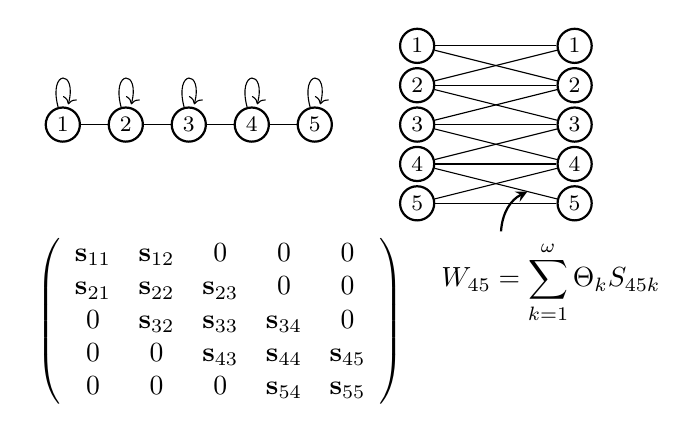
\begin{tikzpicture}
      \tikzstyle{every node} = [draw, circle, thick, inner sep = 2pt]
      \begin{scope}[yshift=3.5cm,xshift=-3cm]
        \foreach \y in {0,...,4}{
          \pgfmathtruncatemacro{\yplusone}{\y + 1}
          
          \node(\y) at (.8*\y,0) {\footnotesize\yplusone};
        }
        \path
        (0) edge[loop above] (0)
        edge (1);
        \path
        (1) edge[loop above] (1)
        edge (2);
        \path
        (2) edge[loop above] (2)
        edge (3);
        \path
        (3) edge[loop above] (3)
        edge (4);
        \path
        (4) edge[loop above] (4);
      \end{scope}
      \begin{scope}[yshift=2.5cm, xshift=1.5cm]
        \foreach \y in {0,...,4}{
          \pgfmathtruncatemacro{\yplusone}{5 - \y}

          \node(a\y) at (0,.5*\y) {\footnotesize\yplusone};
      }
        \foreach \y in {0,...,4}{
          \pgfmathtruncatemacro{\yplusone}{5 - \y}
                  
          \node(\y) at (2,.5*\y) {\footnotesize\yplusone};
      }
      \path
      (a0) edge (0)
      (a0) edge (1);
      \path
      (a1) edge (0)
      (a1) edge (1)
      (a1) edge (2);
      \path
      (a2) edge (1)
      (a2) edge (2)
      (a2) edge (3);
      \path
      (a3) edge (2)
      (a3) edge (3)
      (a3) edge (4);
      \path
      (a4) edge (3)
      (a4) edge (4);
      \end{scope}
      \tikzstyle{every node} = []
      \node at (-1,1) {$\left(\begin{array}{ccccc}
          \mathbf{s}_{11} & \mathbf{s}_{12} & 0 & 0 & 0\\
          \mathbf{s}_{21} & \mathbf{s}_{22} & \mathbf{s}_{23} & 0 & 0\\
          0 & \mathbf{s}_{32} & \mathbf{s}_{33} & \mathbf{s}_{34} & 0\\
          0 & 0 & \mathbf{s}_{43} & \mathbf{s}_{44} & \mathbf{s}_{45}\\
          0 & 0 & 0 & \mathbf{s}_{54} & \mathbf{s}_{55}
        \end{array}\right)$};
      \node(label) at (3.2,1.5) {$W_{45} = \displaystyle{\sum_{k=1}^{\omega}{\Theta_{k} S_{45 k}}}$};
      \path[>=stealth, ->, thick]
      (label) edge[bend left] (2.9,2.65);
    \end{tikzpicture}
  \end{center}
\end{figure}
\end{frame}

\begin{frame}[c, label=current]
  \frametitle{Neural contraction}

%The \emph{neural contraction} $\wideparen{\cdots}$ is a ternary operation defined as:
\begin{gather*}
\wideparen{\Theta SX}[j,q,b] = \displaystyle \sum_{k=1}^\omega \sum_{p=1}^P \sum_{i=1}^n \Theta[k,p,q] \h{2} S[k,i,j] \h{2} X[i,p,b]\\
% \end{gather*}
% In other words
% \begin{gather*}
g(X) = \wideparen{\Theta SX}
\text{ where } \begin{cases} W_{pq}\h{0}^{ij} = \Theta_{pq}\h{0}^k S_k\h{0}^{ij} \\ g(X)_{jq}\h{0}^b = W_{jq}\h{0}^{ip} X_{ip}\h{0}^{b} \end{cases} \label{eq:ternary}
\end{gather*}


\begin{columns}
    \column{.5\textwidth}

    \begin{center}
    \begin{table}[H]
    \centering
    \begin{tabular}{ccl}
      index & size & description\\
      \hline
      $i$ & $n$ & input neuron\\
      $j$ & $m$ & output neuron\\
      $p$ & $N$ & input channel\\
      $q$ & $M$ & feature map\\
      $k$ & $\omega$ & kernel weight\\
      $b$ & $B$ & batch instance
    \end{tabular}
    \caption{indices}
    \label{tab:ind}
    \end{table}
    \end{center}

    \column{.5\textwidth}

    \begin{center}
    \begin{table}[H]
    \centering
    \begin{tabular}{ccc}
      tensor & shape\\
      \hline
      $\Theta$ & $\omega \times N \times M$\\
      $S$ & $\omega \times n \times m$\\
      $X$ & $n \times N \times B$\\
      $\Theta S$ & $n \times m \times N \times M$\\
      $SX$ & $\omega \times m \times N \times B$\\
      $\Theta X$ & $\omega \times n \times M \times B$\\
      $\wideparen{\Theta SX}$ & $m \times M \times B$
    \end{tabular}
    \caption{shapes}
    \label{tab:mid}
    \end{table}
    \end{center}
    
  \end{columns}
\end{frame}


\begin{frame}[c, label=current]
  \frametitle{Properties}
  This formulation is:
  \begin{itemize}
    \item Linear
    \item Associative
    \item Commutative
    \item Generic (next slide)
  \end{itemize}
  It is explainable as a convolution of graph signals when:
  \begin{itemize}
    \item in supervised application
    \item Either $0$ or $1$ weight per connection ($\mathbf{s_{ij}}$ are one-hot vectors)
  \end{itemize}
  In other cases it can be seen as a linear combination of convolutions.
\end{frame}

\begin{frame}[c, label=current]
  \frametitle{Genericity of ternary representation}
  Given adequate specification of the weight sharing scheme $S$, we can obtain, \eg:
  \begin{itemize}
    \item a dense layer
    \item a partially connected layer
    \item a convolutional layer
    \item a graph convolutional layer (GCN, Kipf et al.)
    \item a graph attention layer (GAT, Velickovic et al.)
    \item a topology-adaptive graph convolution layer (TAGCN, Du et al.)
    \item a mixture model convolutional layer (MOnet, Monti et al.)
    \item a generalized convolution under sparse priors
    \item any partial connectivity pattern, sparse or not
  \end{itemize}
\end{frame}


\begin{frame}[c, label=current]
  \frametitle{Discussion}
  \begin{figure}
  \begin{center}
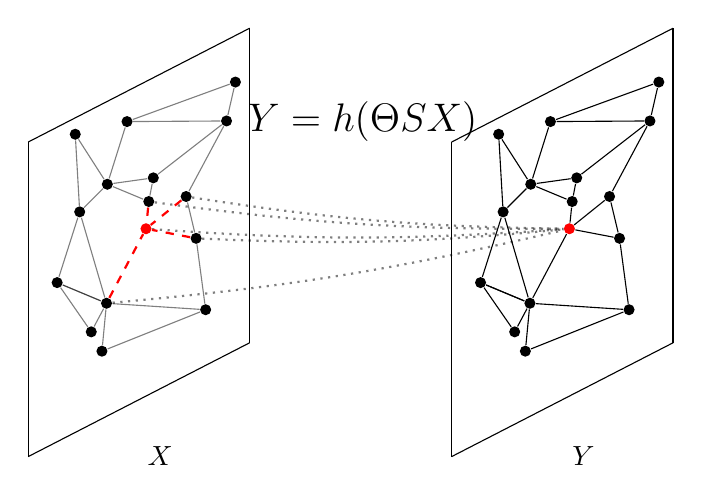
\begin{tikzpicture}[scale=0.85]
  
\newcommand{\nnn}{4.7}
  \begin{scope}[rotate around y = 70]
\pgfmathsetseed{333}
\tikzstyle{every node}= [circle,
fill=black,
 minimum size= 4pt,inner sep=0pt];
    \foreach \x in {1,2,4}{
      \foreach \y in {1,2,3,4}{
        \node(\x\y) at (\x+0.5*rand,\y+0.5*rand) {};
      }
    }
    \foreach \y in {1,2,4}{
        \node(3\y) at (3+0.5*rand,3+0.5*rand) {};
    }
    \node(33)[circle,fill=red] at (2.5,2.5) {};

    \path[thin]
      (0,0) edge (0,\nnn)
      (0,\nnn) edge (\nnn,\nnn)
      (0,0) edge (\nnn,0)
      (\nnn,0) edge (\nnn,\nnn);

    \node[draw=none,fill=none] at (2.8,-1) {$X$};
    \end{scope}
  \begin{scope}[xshift=180pt,rotate around y = 70]
\pgfmathsetseed{333}
\tikzstyle{every node}= [circle,fill=black, minimum size= 4pt,inner sep=0pt];
    \foreach \x in {1,2,4}{
      \foreach \y in {1,2,3,4}{
        \node(\x\y') at (\x+0.5*rand,\y+0.5*rand) {};
      }
    }
    \foreach \y in {1,2,4}{
        \node(3\y') at (3+0.5*rand,3+0.5*rand) {};
    }
    \node(33')[circle,fill=red] at (2.5,2.5) {};

    \path[thin]
      (0,0) edge (0,\nnn)
      (0,\nnn) edge (\nnn,\nnn)
      (0,0) edge (\nnn,0)
      (\nnn,0) edge (\nnn,\nnn);

    \node[draw=none,fill=none] at (2.8,-1) {$Y$};
  \end{scope}
\draw[dotted,thick,-,opacity=0.5] (33) edge[bend right=4] (33');
\draw[dotted,thick,-,opacity=0.5] (22) edge[bend right=4] (33');
\draw[dotted,thick,-,opacity=0.5] (32) edge[bend right=4] (33');
\draw[dotted,thick,-,opacity=0.5] (31) edge[bend right=4] (33');
\draw[dotted,thick,-,opacity=0.5] (42) edge[bend right=4] (33');

\path[thick, dashed, red]
  (22) edge (33)
  (32) edge (33)
  (31) edge (33)
  (42) edge (33);

\path[opacity=0.5]
  (22) edge (13)
  (22) edge (12)
  (22) edge (11)
  (22) edge (21)
  (22) edge (41)
  (21) edge (41)
  (42) edge (31)
  (43) edge (31)
  (43) edge (24)
  (44) edge (43)
  (32) edge (23)
  (32) edge (34)
  (22) edge (12)
  (23) edge (14)
  (11) edge (12)
  (14) edge (13)
  (24) edge (23)
  (34) edge (43)
  (23) edge (34)
  (23) edge (13)
  (12) edge (13)
  (42) edge (41)
  (24) edge (44);

\path[]
  (22') edge (33')
  (32') edge (33')
  (31') edge (33')
  (42') edge (33')
  (22') edge (13')
  (22') edge (12')
  (22') edge (11')
  (22') edge (21')
  (22') edge (41')
  (21') edge (41')
  (42') edge (31')
  (43') edge (31')
  (43') edge (24')
  (44') edge (43')
  (32') edge (23')
  (32') edge (34')
  (22') edge (12')
  (23') edge (14')
  (11') edge (12')
  (14') edge (13')
  (24') edge (23')
  (34') edge (43')
  (23') edge (34')
  (23') edge (13')
  (12') edge (13')
  (42') edge (41')
  (24') edge (44');

  \node at (5,5) {\Large $Y = h(\wideparen{\Theta SX})$};
\end{tikzpicture}
  \end{center}
\end{figure}
The propagation logic is in the scheme S. For example, it can be either:
\begin{multicols}{2}
\begin{itemize}
  \item given
  \item randomized
  \item learned
  \item inferred
\end{itemize}
\end{multicols}
\end{frame}
\section{Experiments}

\begin{frame}[c, label=current]
  \frametitle{Outline}
  Experiments:
    \begin{itemize}
      \item Study of influence of symmetries using $S$
      \item Learning $S$ when masked by an adjacency matrix and its powers
      \item Monte Carlo simulations with random realizations of $S$ 
      \item Learning $S$ in semi-supervised applications
      \item Inferring $S$ from translations
    \end{itemize}
\end{frame}

\begin{frame}[c, label=current]
  \frametitle{Datasets}
    \begin{center}
    \begin{tikzpicture}
    \node at (-3, 4) {\includegraphics[width=0.28\linewidth,height=\textheight,keepaspectratio]{mnistt.png}};
    \node at (1, 4) {\includegraphics[width=0.28\linewidth,height=\textheight,keepaspectratio]{cifart.png}};
    \node at (5, 4) {\includegraphics[width=0.28\linewidth,height=\textheight,keepaspectratio]{cifartscrambled.png}};
    \node at (-3, 0) {\includegraphics[width=0.3\linewidth,height=\textheight,keepaspectratio]{brain.jpeg}};
    \node at (1, 0) {\includegraphics[width=0.3\linewidth,height=\textheight,keepaspectratio]{embedding.png}};
    \node at (5, 0) {\includegraphics[width=0.3\linewidth,height=\textheight,keepaspectratio]{citationNet.png}};
    \end{tikzpicture}
    \end{center}
\end{frame}

\begin{frame}[c, label=current]
  \frametitle{Influence of symmetries}
  %\centering{\Large $Y = h(\wideparen{\textcolor{orange}{\Theta} \textcolor{blue}{S} X})$}
  \centering{\Large $Y = h(\wideparen{\textcolor{orange}{\Theta} \textcolor{blue}{S}X})$}
  \begin{center}
  \begin{tikzpicture}
  \node at (0, 4) {\includegraphics[width=0.4\linewidth,height=\textheight,keepaspectratio]{rregular.pdf}};
  \node at (5, 4) {\includegraphics[width=0.4\linewidth,height=\textheight,keepaspectratio]{iirregular.pdf}};
  \end{tikzpicture}
  \end{center}
\end{frame}


\begin{frame}[c, label=current]
  \frametitle{Influence of symmetries: results on MNIST}
  \centering{\Large $Y = h(\wideparen{\textcolor{orange}{\Theta} \textcolor{blue}{S} X})$}
\begin{figure}
  \centering
  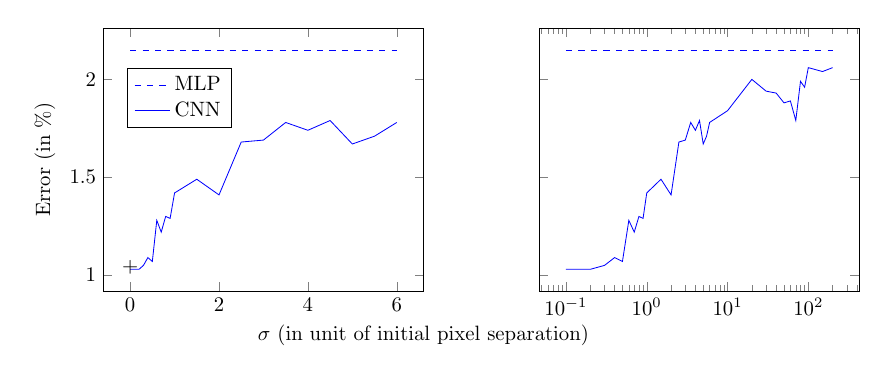
\begin{tikzpicture}[scale=0.75]
    \begin{axis}[xlabel=$\sigma$ (in unit of initial pixel separation), ylabel=Error (in \%),
      legend style={at={(0.4,0.85)}, anchor=north east},
      x label style={at={(axis description cs:1,-0.1)},anchor=north}]

      \addplot[color=blue,dashed,mark=.] coordinates {
        (0.0, 2.15) (6.0, 2.15)
      };

      \addplot[color=blue,mark=.] coordinates {
      (0.0, 1.03)
      (0.1, 1.03)
      (0.2, 1.03)
      (0.3, 1.05)
      (0.4, 1.09)
      (0.5, 1.07)
      (0.6, 1.28)
      (0.7, 1.22)
      (0.8, 1.30)
      (0.9, 1.29)
      (1.0, 1.42)
      (1.5, 1.49)
      (2.0, 1.41)
      (2.5, 1.68)
      (3.0, 1.69)
      (3.5, 1.78)
      (4.0, 1.74)
      (4.5, 1.79)
      (5.0, 1.67)
      (5.5, 1.71)
      (6.0, 1.78)
      };

      \node at (0.0, 1.03) {+};
      %\node at (0.0, 1.10) {\scriptsize{CNN}};

      \legend{MLP, CNN}
    \end{axis}

    \begin{scope}[xshift = 210pt]
      \begin{semilogxaxis}[yticklabels={,,}]

        %\node at (0.1, 1.49) {+};

        \addplot[color=blue,mark=.] coordinates {
        (0.0, 1.03)
        (0.1, 1.03)
        (0.2, 1.03)
        (0.3, 1.05)
        (0.4, 1.09)
        (0.5, 1.07)
        (0.6, 1.28)
        (0.7, 1.22)
        (0.8, 1.30)
        (0.9, 1.29)
        (1.0, 1.42)
        (1.5, 1.49)
        (2.0, 1.41)
        (2.5, 1.68)
        (3.0, 1.69)
        (3.5, 1.78)
        (4.0, 1.74)
        (4.5, 1.79)
        (5.0, 1.67)
        (5.5, 1.71)
        (6.0, 1.78)
        (10.0, 1.84)
        (20.0, 2.00)
        (30.0, 1.94)
        (40.0, 1.93)
        (50.0, 1.88)
        (60.0, 1.89)
        (70.0, 1.79)
        %(75.0, 1.91)
        (80.0, 1.99)
        (90.0, 1.96)
        (100.0, 2.06)
        (150.0, 2.04)
        (200.0, 2.06)
        };

        \addplot[color=blue,dashed,mark=.] coordinates { 
        (0.0, 2.15)
        (0.1, 2.15)
        (200.0, 2.15)
        };

      \end{semilogxaxis}
    \end{scope}

  \end{tikzpicture}
  %\caption{Error in function of the standard deviation $\sigma$, for generalized CNNs and an MLP, each with $500$ weights.}
  \label{fig:expres}
\end{figure}
\end{frame}

% \begin{frame}[c, label=current]
%   \frametitle{Extending GCN in semi-supervised settings}
% \end{frame}

% \begin{frame}[c, label=current]
%   \frametitle{Experiments on MNIST}
%   \centering\includegraphics[width=0.6\linewidth,height=\textheight,keepaspectratio]{mnist5.png}\\
%   \centering\includegraphics[width=0.6\linewidth,height=\textheight,keepaspectratio]{scambled5.png}

%   \begin{itemize}
%   \item 10 categories,
%   \item 60'000 training images,
%   \item 10'000 test images.
%   \end{itemize}
% \end{frame}

\begin{frame}[c, label=current]
  \frametitle{Learning both $S$ and $\Theta$ on MNIST and scrambled MNIST}
  \centering{\Large $Y = h(\wideparen{\textcolor{orange}{\Theta} \textcolor{orange}{S} X})$}
  \begin{table}[h]
  \begin{center}
    \bgroup
    \def\arraystretch{1.5}%  1 is the default, change whatever you need
    \begin{tabular}{|c|c|c|c|c|c|c|c|}
      \hline
      Ordering & Conv5x5 & $A^1$ & $A^2$ & $A^3$ & $A^4$ & $A^5$ & $A^6$\\
      \hline
      no prior & / & 1.24\% & 1.02\% & 0.93\% & 0.90\% & 0.93\% & 1.00\%\\
      \hline
      prior & 0.87\% & 1.21\% & 0.91\% & 0.91\% & 0.87\% & 0.80\% & 0.74\%\\
      \hline
    \end{tabular}
    \egroup
  \end{center}
  \caption{Grid graphs on MNIST}
\end{table}
\pause
\begin{table}[h]
  %\caption{Error rates when topology is unknown on scrambled MNIST.}
  \begin{center}
    \bgroup
    \def\arraystretch{1.5}%  1 is the default, change whatever you need
    \begin{tabular}{|c|c|c|c|}
      \hline
      MLP & Conv5x5 & Thresholded ($p=3\%$) & $k$-NN ($k=25$)\\
      \hline
      1.44\% & 1.39\% & 1.06\% & 0.96\%\\
      \hline
    \end{tabular}
    \egroup
  \end{center}
  \caption{Covariance graphs on Scrambled MNIST}
  \end{table}
\end{frame}

\begin{frame}[c, label=current]
  \frametitle{Experiments on text categorization}
  \centering{\Large $Y = h(\wideparen{\textcolor{orange}{\Theta} \textcolor{blue}{S} X})$}
  \begin{figure}

\centering

    \scalebox{0.6}{
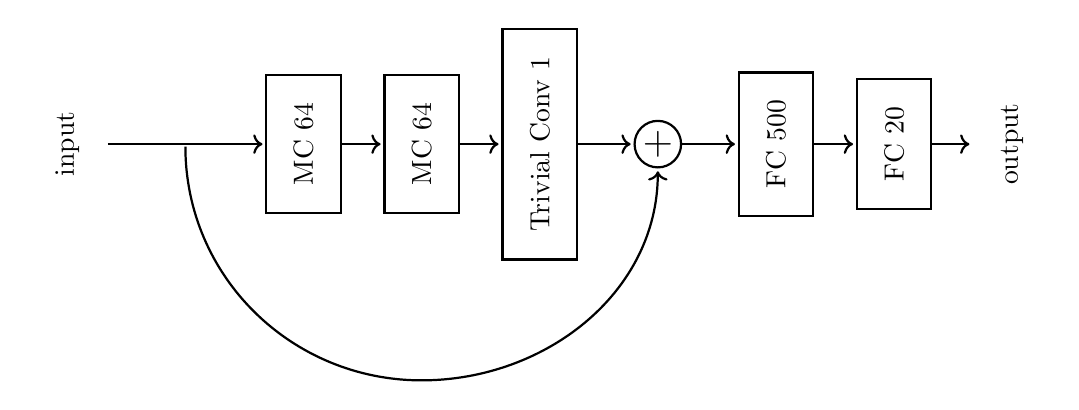
\begin{tikzpicture}[shorten >=1pt,node distance=1.5cm, thick]
   \tikzstyle{every node} = [inner sep=10pt, transform shape];
   \begin{scope}[rotate=90]
     \node[]   (a)                {input};
     \node[]           (b) [below of = a, inner sep=0pt] {};
     \node[rectangle, draw]           (c) [below of = b] {MC $64$};
     \node[rectangle, draw]           (d) [below of = c] {MC $64$};
     \node[rectangle, draw]           (e) [below of = d] {Trivial Conv $1$};
     \node[circle, draw, inner sep=0.03cm] (f) [below of = e] {\Large{+}};
     \node[rectangle, draw]           (g) [below of = f] {FC $500$};
     \node[rectangle, draw]           (h) [below of = g] {FC $20$};
     \node[]           (i) [below of = h] {output};
     \path[->] (a) edge (c);
     \path[->] (c) edge (d);
     \path[->] (d) edge (e);
     \path[->] (e) edge (f);
     \path[->] (f) edge (g);
     \path[->] (g) edge (h);
     \path[->] (h) edge (i);
     \draw[->] (b) to[out=180, in=90] ($(d) - (3,0)$) to[in=180,out=270] (f);
   \end{scope}
\end{tikzpicture}}
\caption{Diagram of the MCNet architecture used}
\label{fig:archiMC}
\end{figure}

\begin{table}[H]
  \begin{center}
    \bgroup
    \def\arraystretch{1.5}%  1 is the default, change whatever you need
    \begin{tabular}{|c|c|c|c|c|c|}
      \hline
      MNB & FC2500 & FC2500-500 & ChebNet32 & FC500 & MCNet\\
      \hline
      $68.51$ & $64.64$ & $65.76$ & $68.26$ & $71.46\h{2}(72.25)$ & $70.74\h{2}(\mathbf{72.62})$\\
      \hline
    \end{tabular}
    \egroup
  \end{center}
  \label{tab:20}
  \caption{Accuracies (in \%) on $20$NEWS, given as \textit{mean (max)}}
\end{table}

\end{frame}


% \begin{frame}[c, label=current]
%   \frametitle{Experiments on citation networks}
%   \centering\includegraphics[width=0.8\linewidth,height=\textheight,keepaspectratio]{citationNet.png}
% \end{frame}


\begin{frame}[c, label=current]
  \frametitle{Benchmarks on citation networks}
  \begin{center}{\Large $Y = h(\wideparen{\textcolor{orange}{\Theta} \textcolor{orange}{S} X})$}\\\end{center}
  Comparison of
  \begin{itemize}%[nolistsep,noitemsep]
     \item Graph Convolution Network (GCN),
     \item Graph Attention Network (GAT),
     \item Topology Adaptive GCN (TAGCN).
  \end{itemize}
  With our models:
  \begin{itemize}
     \item Addition of graph dropout to GCN (GCN*),
     \item Graph Contraction Network (GCT).
\end{itemize}
\begin{small}
  \begin{table}[h]
  \begin{center}
    \bgroup
    \def\arraystretch{1.5}%  1 is the default, change whatever you need
    \begin{tabular}{|c|c|c|c|c|c|c|}
    \hline
    \small{Dataset} & MLP & GCN & GAT & TAGCN & GCN* & GCT\\
    \hline
    \hline
    \small{Cora} & $58.8 \pm 0.9$ & $81.8 \pm 0.9$ & $83.3 \pm 0.6$ & $82.9 \pm 0.7$ & $\mathbf{83.4} \pm 0.7$ & $83.3 \pm 0.7$\\
    \hline
    \small{Citeseer} & $56.7 \pm 1.1$ & $72.2 \pm 0.6$ & $72.1 \pm 0.6$ & $71.7 \pm 0.7$ & $72.5 \pm 0.8$ & $\mathbf{72.7} \pm 0.5$\\
    \hline
    \small{Pubmed} & $72.6 \pm 0.9$ & $79.0 \pm 0.5$ & $78.3 \pm 0.7$ & $78.9 \pm 0.5$ & $78.2 \pm 0.7$ & $\mathbf{79.2} \pm 0.4$\\
    \hline
  \end{tabular}
    \egroup
  \end{center}
  \caption{Mean accuracy (in \%) and standard deviation after $100$ run}
  \end{table}
\end{small}
\end{frame}

\begin{frame}
  \frametitle{Another approach: finding translations in graphs to construct $S$}
  Step 0 : infer a graph
  \begin{center}
    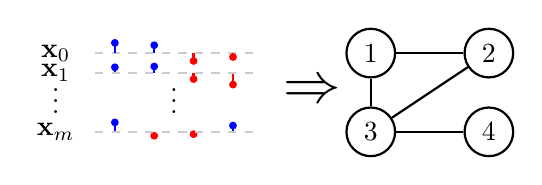
\begin{tikzpicture}[thick]
      \node at (0,0) {$\mathbf{x}_0$};
      \path[black!20!white, dashed]
      (0.5,0) edge (2.5,0);
      \path
      (0.75, 0) edge[blue] (0.75, 0.13)
      (1.25, 0) edge[blue] (1.25, 0.1)
      (1.75, 0) edge[red] (1.75, -0.1)
      (2.25, 0) edge[red] (2.25, -0.05);
      \node[fill, circle, inner sep = 1pt, blue] at (0.75, 0.13) {};
      \node[fill, circle, inner sep = 1pt, blue] at (1.25, 0.1) {};
      \node[fill, circle, inner sep = 1pt, red] at (1.75, -0.1) {};
      \node[fill, circle, inner sep = 1pt, red] at (2.25, -0.05) {};
      \node at (0,-0.25) {$\mathbf{x}_1$};
      \begin{scope}[yshift=-0.25cm]
        \path
        (0.75, 0) edge[blue] (0.75, 0.07)
        (1.25, 0) edge[blue] (1.25, 0.08)
        (1.75, 0) edge[red] (1.75, -0.08)
        (2.25, 0) edge[red] (2.25, -0.15);
        \node[fill, circle, inner sep = 1pt,blue] at (0.75, 0.07){};
        \node[fill, circle, inner sep = 1pt,blue] at (1.25, 0.08){};
        \node[fill, circle, inner sep = 1pt,red] at (1.75, -0.08){};
        \node[fill, circle, inner sep = 1pt,red] at (2.25, -0.15){};        
      \end{scope}

      \path[black!20!white, dashed]
      (0.5,-0.25) edge (2.5,-0.25);
      \node at (0,-0.5) {\vdots};
      \node at (0,-1) {$\mathbf{x}_m$};
      \begin{scope}[yshift=-1cm]
        \path
        (0.75, 0) edge[blue] (0.75, 0.12)
        (1.25, 0) edge[red] (1.25, -0.05)
        (1.75, 0) edge[red] (1.75, -0.03)
        (2.25, 0) edge[blue] (2.25, 0.08);
        \node[fill, circle, inner sep = 1pt, blue] at (0.75, 0.12){};
        \node[fill, circle, inner sep = 1pt, red] at (1.25, -0.05){};
        \node[fill, circle, inner sep = 1pt, red] at (1.75, -0.03){};
        \node[fill, circle, inner sep = 1pt, blue] at (2.25, 0.08){};        
      \end{scope}
      \node at (1.5,-0.5) {\vdots};
      \path[black!20!white, dashed]
      (0.5,-1) edge (2.5,-1);

      \node at (3.25, -0.5) {\huge{$\Rightarrow$}};

      \begin{scope}[xshift=4cm]
        \node[draw, circle](a) at (0,0) {1};
        \node[draw, circle](b) at (1.5,0) {2};
        \node[draw, circle](c) at (1.5,-1) {4};
        \node[draw, circle](d) at (0,-1) {3};
      \end{scope}
      \path
      (a) edge (b)
      edge (d)
      (b) edge (d)
      (c) edge (d);
    \end{tikzpicture}
  \end{center}
  \pause
  Step 1: infer translations
  \begin{center}
    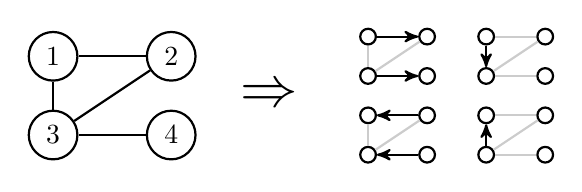
\begin{tikzpicture}[thick]      
      \begin{scope}[xshift=0cm]
        \node[draw, circle](a) at (0,0) {1};
        \node[draw, circle](b) at (1.5,0) {2};
        \node[draw, circle](c) at (1.5,-1) {4};
        \node[draw, circle](d) at (0,-1) {3};
      \end{scope}
      \path
      (a) edge (b)
      edge (d)
      (b) edge (d)
      (c) edge (d);
      \node at (2.75, -0.5) {\huge{$\Rightarrow$}};
      \begin{scope}[xshift=4cm, scale=0.5, yshift=0.5cm]
        \node[draw, inner sep=2pt, circle](a) at (0,0) {};
        \node[draw, inner sep=2pt, circle](b) at (1.5,0) {};
        \node[draw, inner sep=2pt, circle](c) at (1.5,-1) {};
        \node[draw, inner sep=2pt, circle](d) at (0,-1) {};
      \end{scope}
      \path[black!20!white]
      (a) edge (b)
      edge (d)
      (b) edge (d)
      (c) edge (d);
      \path[->,>=stealth']
      (a) edge (b)      
      (d) edge (c);
      \begin{scope}[xshift=4cm, scale=0.5, yshift=-1.5cm]
        \node[draw, inner sep=2pt, circle](a) at (0,0) {};
        \node[draw, inner sep=2pt, circle](b) at (1.5,0) {};
        \node[draw, inner sep=2pt, circle](c) at (1.5,-1) {};
        \node[draw, inner sep=2pt, circle](d) at (0,-1) {};
      \end{scope}
      \path[black!20!white]
      (a) edge (b)
      edge (d)
      (b) edge (d)
      (c) edge (d);
      \path[->,>=stealth']
      (b) edge (a)      
      (c) edge (d);
      \begin{scope}[xshift=5.5cm, scale=0.5, yshift=0.5cm]
        \node[draw, inner sep=2pt, circle](a) at (0,0) {};
        \node[draw, inner sep=2pt, circle](b) at (1.5,0) {};
        \node[draw, inner sep=2pt, circle](c) at (1.5,-1) {};
        \node[draw, inner sep=2pt, circle](d) at (0,-1) {};
      \end{scope}
      \path[black!20!white]
      (a) edge (b)
      edge (d)
      (b) edge (d)
      (c) edge (d);
      \path[->,>=stealth']
      (a) edge (d);
      \begin{scope}[xshift=5.5cm, scale=0.5, yshift=-1.5cm]
        \node[draw, inner sep=2pt, circle](a) at (0,0) {};
        \node[draw, inner sep=2pt, circle](b) at (1.5,0) {};
        \node[draw, inner sep=2pt, circle](c) at (1.5,-1) {};
        \node[draw, inner sep=2pt, circle](d) at (0,-1) {};
      \end{scope}
      \path[black!20!white]
      (a) edge (b)
      edge (d)
      (b) edge (d)
      (c) edge (d);
      \path[->,>=stealth']
      (d) edge (a);
    \end{tikzpicture}
  
  \end{center}
  
\end{frame}
\begin{frame}\frametitle{Another approach: finding translations in graphs to construct $S$}



  Step 2: design convolution weight-sharing

    \begin{center}
    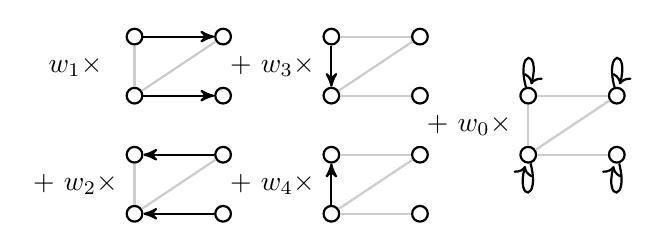
\begin{tikzpicture}[thick]      
      \begin{scope}[xshift=0cm, scale=0.75, yshift=0.5cm]
        \node[inner sep=2pt](w) at (-1.0,-0.5) {$w_1 \times$};
        \node[draw, inner sep=2pt, circle](a) at (0,0) {};
        \node[draw, inner sep=2pt, circle](b) at (1.5,0) {};
        \node[draw, inner sep=2pt, circle](c) at (1.5,-1) {};
        \node[draw, inner sep=2pt, circle](d) at (0,-1) {};       
      \end{scope}
      \path[black!20!white]
      (a) edge (b)
      edge (d)
      (b) edge (d)
      (c) edge (d);
      \path[->,>=stealth']
      (a) edge (b)      
      (d) edge (c);
      \begin{scope}[xshift=0cm, scale=0.75, yshift=-1.5cm]
        \node[inner sep=2pt](w) at (-1.0,-0.5) {+ $w_2 \times$};
        \node[draw, inner sep=2pt, circle](a) at (0,0) {};
        \node[draw, inner sep=2pt, circle](b) at (1.5,0) {};
        \node[draw, inner sep=2pt, circle](c) at (1.5,-1) {};
        \node[draw, inner sep=2pt, circle](d) at (0,-1) {};
      \end{scope}
      \path[black!20!white]
      (a) edge (b)
      edge (d)
      (b) edge (d)
      (c) edge (d);
      \path[->,>=stealth']
      (b) edge (a)      
      (c) edge (d);
      \begin{scope}[xshift=2.5cm, scale=0.75, yshift=0.5cm]
        \node[inner sep=2pt](w) at (-1.0,-0.5) {+ $w_3 \times$};
        \node[draw, inner sep=2pt, circle](a) at (0,0) {};
        \node[draw, inner sep=2pt, circle](b) at (1.5,0) {};
        \node[draw, inner sep=2pt, circle](c) at (1.5,-1) {};
        \node[draw, inner sep=2pt, circle](d) at (0,-1) {};
      \end{scope}
      \path[black!20!white]
      (a) edge (b)
      edge (d)
      (b) edge (d)
      (c) edge (d);
      \path[->,>=stealth']
      (a) edge (d);
      \begin{scope}[xshift=2.5cm, scale=0.75, yshift=-1.5cm]
        \node[inner sep=2pt](w) at (-1.0,-0.5) {+ $w_4 \times$};      
        \node[draw, inner sep=2pt, circle](a) at (0,0) {};
        \node[draw, inner sep=2pt, circle](b) at (1.5,0) {};
        \node[draw, inner sep=2pt, circle](c) at (1.5,-1) {};
        \node[draw, inner sep=2pt, circle](d) at (0,-1) {};
      \end{scope}
      \path[black!20!white]
      (a) edge (b)
      edge (d)
      (b) edge (d)
      (c) edge (d);
      \path[->,>=stealth']
      (d) edge (a);

      \begin{scope}[xshift=5.0cm, scale=0.75, yshift=-0.5cm]
        \node[inner sep=2pt](w) at (-1.0,-0.5) {+ $w_0 \times$};
        \node[draw, inner sep=2pt, circle](a) at (0,0) {};
        \node[draw, inner sep=2pt, circle](b) at (1.5,0) {};
        \node[draw, inner sep=2pt, circle](c) at (1.5,-1) {};
        \node[draw, inner sep=2pt, circle](d) at (0,-1) {};
      \end{scope}
      \path[black!20!white]
      (a) edge (b)
      edge (d)
      (b) edge (d)
      (c) edge (d);
      \path[]
      (a) edge [loop above] (a)
      (b) edge [loop above] (b)
      (c) edge [loop below] (c)
      (d) edge [loop below] (d);

    \end{tikzpicture}
  
  \end{center}
  \pause
  Step 3: design data-augmentation
  \begin{center}
    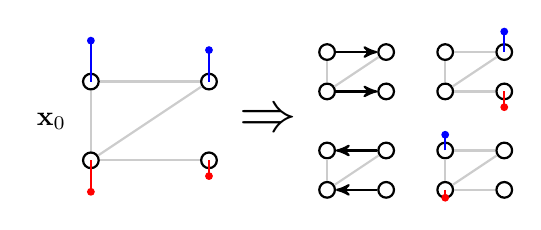
\begin{tikzpicture}[thick]      
      \begin{scope}[xshift=0cm]
        \node[draw, inner sep = 2pt, circle](a) at (0,0) {};
        \node[draw, inner sep = 2pt, circle](b) at (1.5,0) {};
        \node[draw, inner sep = 2pt, circle](c) at (1.5,-1) {};
        \node[draw, inner sep = 2pt, circle](d) at (0,-1) {};
        \path[]
        (0, 0) edge[blue] (0, 0.52)
        (1.5, 0) edge[blue] (1.5, 0.4)
        (0, -1) edge[red] (0, -1.4)
        (1.5, -1) edge[red] (1.5, -1.2);
        \node[fill, circle, inner sep = 1pt, blue] at (0, 0.52) {};
        \node[fill, circle, inner sep = 1pt, blue] at (1.5, 0.4) {};
        \node[fill, circle, inner sep = 1pt, red] at (0, -1.4) {};
        \node[fill, circle, inner sep = 1pt, red] at (1.5, -1.2) {};
      \end{scope}
      \node at (-0.5,-0.5) {$\mathbf{x}_0$};
      \path[black!20!white]
      (a) edge (b)
      edge (d)
      (b) edge (d)
      (c) edge (d);
      \node at (2.25, -0.5) {\huge{$\Rightarrow$}};
      \begin{scope}[xshift=3cm, scale=0.5, yshift=0.75cm]
        \node[draw, inner sep=2pt, circle](a) at (0,0) {};
        \node[draw, inner sep=2pt, circle](b) at (1.5,0) {};
        \node[draw, inner sep=2pt, circle](c) at (1.5,-1) {};
        \node[draw, inner sep=2pt, circle](d) at (0,-1) {};
      \end{scope}
      \path[black!20!white]
      (a) edge (b)
      edge (d)
      (b) edge (d)
      (c) edge (d);
      \path[->,>=stealth']
      (a) edge (b)      
      (d) edge (c);
      \begin{scope}[xshift=4.5cm, scale=0.5, yshift = 0.75cm]
        \node[draw, inner sep = 2pt, circle](a) at (0,0) {};
        \node[draw, inner sep = 2pt, circle](b) at (1.5,0) {};
        \node[draw, inner sep = 2pt, circle](c) at (1.5,-1) {};
        \node[draw, inner sep = 2pt, circle](d) at (0,-1) {};
        \path[]
        (1.5, 0) edge[blue] (1.5, 0.52)
        %% (1.5, 0) edge[blue] (1.5, 0.4)
        (1.5, -1) edge[red] (1.5, -1.4);
        %% (1.5, -1) edge[red] (1.5, -1.2);
        \node[fill, circle, inner sep = 1pt, blue] at (1.5, 0.52) {};
        %% \node[fill, circle, inner sep = 1pt, blue] at (1.5, 0.4);
        \node[fill, circle, inner sep = 1pt, red] at (1.5, -1.4) {};
        %% \node[fill, circle, inner sep = 1pt, red] at (1.5, -1.2);
        \path[black!20!white]
      (a) edge (b)
      edge (d)
      (b) edge (d)
      (c) edge (d);
      \end{scope}      
      \begin{scope}[xshift=3cm, scale=0.5, yshift=-1.75cm]
        \node[draw, inner sep=2pt, circle](a) at (0,0) {};
        \node[draw, inner sep=2pt, circle](b) at (1.5,0) {};
        \node[draw, inner sep=2pt, circle](c) at (1.5,-1) {};
        \node[draw, inner sep=2pt, circle](d) at (0,-1) {};
      \end{scope}
      \path[black!20!white]
      (a) edge (b)
      edge (d)
      (b) edge (d)
      (c) edge (d);
      \path[->,>=stealth']
      (b) edge (a)      
      (c) edge (d);
      \begin{scope}[xshift=4.5cm, scale=0.5, yshift=-1.75cm]
        \node[draw, inner sep = 2pt, circle](a) at (0,0) {};
        \node[draw, inner sep = 2pt, circle](b) at (1.5,0) {};
        \node[draw, inner sep = 2pt, circle](c) at (1.5,-1) {};
        \node[draw, inner sep = 2pt, circle](d) at (0,-1) {};
        \path[]
        %% (0, 0) edge[blue] (0, 0.52)
        (0, 0) edge[blue] (0, 0.4)
        %% (0, -1) edge[red] (0, -1.4)
        (0, -1) edge[red] (0, -1.2);
        %% \node[fill, circle, inner sep = 1pt, blue] at (0, 0.52);
        \node[fill, circle, inner sep = 1pt, blue] at (0, 0.4) {};
        %% \node[fill, circle, inner sep = 1pt, red] at (0, -1.4);
        \node[fill, circle, inner sep = 1pt, red] at (0, -1.2) {};
        \path[black!20!white]
      (a) edge (b)
      edge (d)
      (b) edge (d)
      (c) edge (d);
      \end{scope}
    \end{tikzpicture}
    
  \end{center}
\end{frame}

  \begin{frame}
  \frametitle{Another approach: finding translations in graphs to construct $S$}
  Step 4: design graph subsampling and convolution weight-sharing
  \begin{center}
    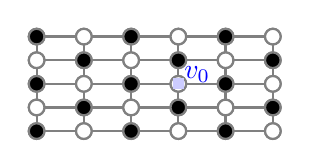
\begin{tikzpicture}[thick, scale=0.6]
      \tikzstyle{every node} = [inner sep = 2pt];
      \foreach \x in {0,...,5}{
        \foreach \y in {0,...,4}{
          \node [draw, circle, black!50] at (\x, \y/2) {};
        }
      }
      \foreach \x in {0,...,4}{
        \foreach \y in {0,...,4}{
          \path[-]
          (\x,\y/2) edge[black!50] (\x+1,\y/2);
        }
      }
      \foreach \x in {0,...,5}{
        \foreach \y in {0,...,3}{
          \path[-]
          (\x,\y/2) edge[black!50] (\x,\y/2 + 1/2);
        }
      }
      \foreach \x in {0,...,5}{
        \foreach \y in {0,...,4}{
          \pgfmathtruncatemacro{\sum}{\x+\y}
          \ifodd\sum
          \node(\x\y) [draw = black!50, circle,fill=white] at (\x, \y/2) {};
          \else
          \node(\x\y) [draw = black!50, circle,fill=black] at (\x, \y/2) {};
          \fi
        }
      }
      \node at (3.4,1.2){\textcolor{blue}{$v_0$}};
      \node[fill=blue!20!white] at (3,1){};
    \end{tikzpicture}
\end{center}
  \begin{center}
    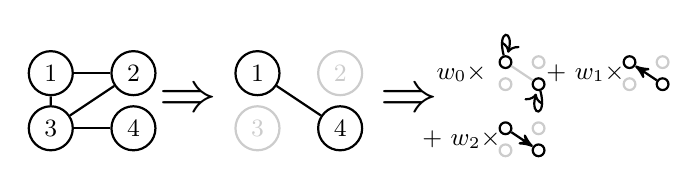
\begin{tikzpicture}[thick, scale=0.7]
      \tikzstyle{every node} = [inner sep = 3pt];
      \small{\begin{scope}[xshift=-0.5cm]
        \node[draw, circle](a) at (0,0) {1};
        \node[draw, circle](b) at (1.5,0) {2};
        \node[draw, circle](c) at (1.5,-1) {4};
        \node[draw, circle](d) at (0,-1) {3};
      \end{scope}
      \path
      (a) edge (b)
      edge (d)
      (b) edge (d)
      (c) edge (d);
      \node at (2, -0.5) {\huge{$\Rightarrow$}};
      \begin{scope}[xshift=3.25cm]
        \node[draw, circle](a) at (0,0) {1};
        \node[draw, circle, black!20!white](b) at (1.5,0) {2};
        \node[draw, circle](c) at (1.5,-1) {4};
        \node[draw, circle, black!20!white](d) at (0,-1) {3};
      \end{scope}
      \path
      (a) edge (c);
      \node at (6, -0.5) {\huge{$\Rightarrow$}};
      \begin{scope}[xshift=7.75cm, scale=0.4, yshift=0.5cm]
        \node[inner sep=1pt](w) at (-2.0,-0.5) {$w_0 \times$};
        \node[draw, inner sep=1.5pt, circle](a) at (0,0) {};
        \node[draw, inner sep=1.5pt, circle, black!20!white](b) at (1.5,0) {};
        \node[draw, inner sep=1.5pt, circle](c) at (1.5,-1) {};
        \node[draw, inner sep=1.5pt, circle, black!20!white](d) at (0,-1) {};
      \end{scope}
      \path[black!20!white]
      (a) edge (c);
      \path[]
      (a) edge [loop above] (a)
      (c) edge [loop below] (c);
      \begin{scope}[xshift=10cm, scale=0.4, yshift=0.5cm]
        \node[inner sep=1pt](w) at (-2.0,-0.5) {+ $w_1 \times$};
        \node[draw, inner sep=1.5pt, circle](a) at (0,0) {};
        \node[draw, inner sep=1.5pt, circle, black!20!white](b) at (1.5,0) {};
        \node[draw, inner sep=1.5pt, circle](c) at (1.5,-1) {};
        \node[draw, inner sep=1.5pt, circle, black!20!white](d) at (0,-1) {};
      \end{scope}
      \path[black!20!white]
      (a) edge (c);
      \path[]
      (c) edge [->,>=stealth'] (a);

      \begin{scope}[xshift=7.75cm, scale=0.4, yshift=-2.5cm]
        \node[inner sep=1pt](w) at (-2.0,-0.5) {+ $w_2 \times$};
        \node[draw, inner sep=1.5pt, circle](a) at (0,0) {};
        \node[draw, inner sep=1.5pt, circle, black!20!white](b) at (1.5,0) {};
        \node[draw, inner sep=1.5pt, circle](c) at (1.5,-1) {};
        \node[draw, inner sep=1.5pt, circle, black!20!white](d) at (0,-1) {};
      \end{scope}
      \path[black!20!white]
      (a) edge (c);
      \path[->,>=stealth']
      (a) edge [] (c);
  
      }
    \end{tikzpicture}
  
\end{center}
\end{frame}

% \begin{frame}
%   \frametitle{Scrambled CIFAR-10 experiments}
%   \begin{center}
%     \includegraphics[width=.5\textwidth]{cifarexamples.png}
%   \end{center}
%   \begin{itemize}
%   \item 10 categories,
%   \item 60'000 training images,
%   \item 10'000 test images.
%   \end{itemize}
% \end{frame}

% \begin{frame}
%   \frametitle{Data augmentation example}
%   \begin{center}
%     \begin{tabular}{cc}
%       Initial image & Random crop \\
      
%       \includegraphics[width=3cm]{truck.png} &


%       \includegraphics[width=3cm]{truck_crop.png}\\

%       Covariance graph & Grid graph\\
      
%       \includegraphics[width=3cm]{truck_graph.png} &


%       \includegraphics[width=3cm]{truck_grid.png}
%     \end{tabular}
%   \end{center}
    
% \end{frame}

\begin{frame}[c, label=current]
  \frametitle{Architecture}
  We used a variant of deep residual networks (ResNet).\\
  We swap operations (data augmentation, convolutions, subsampling) with their counterparts.
  \begin{center}
  \includegraphics[width=\textwidth,height=\textheight,keepaspectratio]{resnet.png}
  \end{center}
\end{frame}

\begin{frame}
  \frametitle{Results on CIFAR-10, scrambled CIFAR-10 and PINES fMRI}
  \centering{\Large $Y = h(\wideparen{\textcolor{orange}{\Theta} \textcolor{blue}{S} X})$}
\begin{table}[h!]
\begin{center}
\vspace{-0.4cm}
\label{tab:cifar-table}
\resizebox{\columnwidth}{!}{%
\begin{tabular}{|l|c|c|c|c|c|}
\hline
\multirow{2}{*}{Support} & \multirow{2}{*}{MLP} %\multirow{2}{*}{\begin{tabular}[c]{@{}c@{}}MLP \\\citeauthor{lin2015}\end{tabular}}
& \multirow{2}{*}{CNN} & \multicolumn{2}{c|}{Grid Graph}       & Covariance Graph         \\ \cline{4-6} 
                         &                                                                                &                      & ChebNet$^c$ & Proposed & Proposed              \\ \hline
Full Data Augmentation   & 78.62\%$^{a,b}$                                                                     & \textbf{93.80\%}     & 85.13\%                            & 93.94\%  & 92.57\%                                         \\ \hline
Data Augmentation w/o Flips & ------                                                                         & 92.73\%              & 84.41\%                            & 92.94\%  & 91.29\%                                         \\ \hline
Graph Data Augmentation  & ------                                                                         & 92.10\%$^d$          & ------                             & 92.81\%  & \textbf{91.07\%}$^a$                             \\ \hline
None                     & 69.62\%                                                                        & 87.78\%              & ------                             & 88.83\%  & 85.88\%$^a$                                      \\\hline
\end{tabular}

}
%\vspace{-0.2cm}
\end{center}
\begin{flushleft}
\footnotesize{
$^a$ No priors about the structure\\
$^b$ Lin et al., 2015\\
$^c$ Defferard et al., 2016\\
$^d$ Data augmentation done with covariance graph 
}
\end{flushleft}
\caption{CIFAR-10 and scrambled CIFAR-10}
\end{table}

\pause

  \begin{table}[h!]
\centering
\label{tab:iaps-table}
\begin{tabular}{|l||c|c||c|c|}
\hline
\multicolumn{1}{|l||}{Support} & \multicolumn{2}{c||}{None} & \multicolumn{2}{c|}{Neighborhood Graph}     \\ \hline
Method                      & MLP & CNN (1x1 kernels)                                & ChebNet$^c$ & Proposed                   \\ \hline
Accuracy                    & 82.62\% & 84.30\%                            & 82.80\%                            & \textbf{85.08\%} \\ \hline
\end{tabular}
%\vspace{-.4cm}
\caption{PINES fMRI}
\end{table}
\end{frame}

\section{Conclusion}

\begin{frame}[c, label=current]
  We studied convolutions of graph signals and used them to build and understand extensions of CNN on graph domains.\\
  \h{0}\\
  \frametitle{Summary}
  Convolution of graph signals:
  \begin{itemize}
    \item Algebraic description of convolution of graph signals $\varphi$- and $\M$-convolutions,
    \item Constructed as the class of linear operator that are equivariant to actions of a group.
    \item Strong characterization results for graphs with Cayley subgraphs.
    \item Extension with groupoids.
  \end{itemize}
  Deep learning on graphs:
  \begin{itemize}
    \item Novel representation based on weight sharing: the neural contraction
    \item Monte-Carlo Neural Networks (MCNN)
    \item Graph Contraction Networks (GCT)
    \item Graph dropout (GCN*)
    \item Translation-Convolutional Neural Network (TCNN)
  \end{itemize}
\end{frame}

\begin{frame}[c, label=current]
  \frametitle{Final words}

  Perspectives:
  \begin{itemize}
    \item In the literature of this domain: semi-supervised $>>$ supervised.
    \item Both tasks can be abstracted to a more general case.
    $$
    Y = h(\wideparen{\Theta S X})
    $$
    \item There can be more than one tensor rank which relations can be represented by a graph.
    $$
    Y = h(g(X, A_1, A_2, ..., A_r))
    $$
    \item Extended range of applications for deep learning architecture.
    \item Thinking in AI might be about creating connections (captured by $S$) and not about updating weights.
  \end{itemize}
  \h{0}\\\h{0}\\
\begin{center}
  {\Large Thank you for your attention !}
\end{center}
\end{frame}

\begin{frame}[c, label=current]
 \frametitle{Contributions}
 {\small
  \begin{itemize}
    \item \textbf{Generalizing the convolution operator to extend CNNs to irregular domains}, Jean-Charles Vialatte, Vincent Grippon, Grégoire Mercier, \textit{arXiv preprint 2016}.
    \item \textbf{Neighborhood-preserving translations on graphs}, Nicolas Grelier, Bastien Pasdeloup, Jean-Charles Vialatte, Vincent Gripon, \textit{IEEE GlobalSIP 2016}.
    \item \textbf{Learning local receptive fields and their weight sharing scheme on graphs}, Jean-Charles Vialatte, Vincent Gripon, Gilles Coppin, \textit{IEE GlobalSIP 2017}.
    \item \textbf{A study of deep learning robustness against computation failures}, Jean-Charles Vialatte, François Leduc-Primeau, \textit{ACTA 2017}.
    \item \textbf{Convolutional neural networks on irregular domains through approximate translations on inferred graphs}, Bastien Pasdeloup, Vincent Gripon, Jean-Charles Vialatte, Dominique Pastor, \textit{arXiv preprint 2017}.
    \item \textbf{Translations on graphs with neighborhood preservation}, Bastien Pasdeloup, Vincent Gripon, Nicolas Grelier, Jean-Charles Vialatte, Dominique Pastor, \textit{arXiv preprint 2017}.
    \item \textbf{Matching CNNs without Priors about data}, Carlos-Eduardo Rosar Kos Lassance, Jean-Charles Vialatte, Vincent Gripon, \textit{IEEE DSW 2018}.
    \item \textbf{On convolution of graph signals and deep learning on graph domains}, Jean-Charles Vialatte, thesis, \textit{unpublished}.
    \item \textbf{Convolution of graph signals}, Jean-Charles Vialatte, Vincent Gripon, Gilles Coppin, \textit{unpublished}.
    \item \textbf{Graph contraction networks, Graph dropout, Monte-Carlo Networks}, Jean-Charles Vialatte, Vincent Gripon, Gilles Coppin, \textit{unpublished}.
  \end{itemize}
 }
\end{frame}

\end{document}
